%% Latex template for PhD dissertation or MS thesis
%% Department of Mechanical Engineering
%% Brigham Young University
%% Last Modified: June 2016

%\documentclass[12pt,twoside]{report}% Use this line for the print version of the thesis
\documentclass[12pt,oneside]{report}% If you comment out the line above, and uncomment this line, it will create a file without the extra pages that the Library wants for its electronic file versions.

%%%%%%%%%%%%%%%%%%%%%%%%%%%%%%%%%%%%%%%%%%%%%%%%%%%%%%%%%
%  Setup BYU thesis format
%%%%%%%%%%%%%%%%%%%%%%%%%%%%%%%%%%%%%%%%%%%%%%%%%%%%%%%%%
\usepackage{byustyle}
% Setup the byu style sheet
\byustylesetup{%
    %
    %isdissertation = true,            % Uncomment this if you're doing a PhD dissertation
    %
    % Definitions of names needed in thesis/dissertation
    deptname          = Department of Civil and Environmental Engineering,
    committeechairman = Gregory Macfarlane,
    committeemembera  = Grant G. Schultz,
    committeememberb  = Daniel P. Ames,
    %graddate = December 2021,  		% Final approval month (NOT graduation month!
     %
    %Uncomment to shorten for proofreading purposes
    %noabstract = true,         % Don't show the abstract page
    %nouniversitypages = true,  % Don't show any of the "university pages"
    %noacknowledgements = true, % Don't show the Acknowledgements page
    %notableofcontents = true,  % Don't show the Table of Contents
    %nolistoffigures = true,    % Don't show the List of Figures
   % nolistoftables = true,     % Don't show the List of Tables
    nonomenclature = true,     % Don't show the Nomenclature section - note that this section is optional
    %notocandlists = true,      % Don't show the Table of Contents, List of Figures, or the List of Tables
    %noheaderatall = true,      % Don't show any of the BYU Thesis header pages
    keywords = {resilience, resiliency, logsum, logit model, choice model, mode choice,
    destination choice, transportation model, transportation planning, route path, link vulnerability, cost estimate} % Enter your keywords
%inside the curly braces, as you'd like them to appear on the bottom of the abstract page.
}
%%%%%%%%%%%%%%%%%%%%%%%%%%%%%%%%%%%%%%%%%%%%%%%%%%%%%%%%
%  Include other \usepackage{} statements here.
%    Add one package at a time.
%    Warning:  Some packages are not compatible with byuthesis.sty
%%%%%%%%%%%%%%%%%%%%%%%%%%%%%%%%%%%%%%%%%%%%%%%%%%%%%%%%%
% You should turn on any of these that you think you'll need!

%\usepackage[normalmargins]{savetrees} 	% prints smaller to save trees (draft only)
\usepackage{amsmath}										%	allows for mathematical symbols
\usepackage{amssymb}										%	defines symbol names for all the
%math symbols
\usepackage{graphicx}        						% for .pdf graphics inclusion
%\usepackage{subfigure}									%	allows for subfigures
%\usepackage{adjustbox}
\usepackage{makecell}
\usepackage{caption}
\usepackage[calcwidth = \columnwidth]{caption}
\usepackage{booktabs,threeparttable}
\usepackage{subcaption}
\usepackage{setspace}										%	change the spacing inside a
%document
\usepackage{epstopdf}										%	converts a .eps to a .pdf
\usepackage{natbib}												%	allows for citations
\usepackage{mathptmx}
\usepackage{textcomp}
\usepackage{pdflscape}
\usepackage{float}											%	improves the interface for defining floating objects
\usepackage{rotating}
\newcommand{\squeezeup}{\vspace{-2.5mm}}
%\usepackage[figuresright]{rotfloat}
%\usepackage{multirow}
%These next two lines are for the citing with the IEEE style (leave commented for ASME)
%\renewcommand\citepunct{], [}
%\renewcommand\citedash{]--[}
%%%%%%%%%%%%%%%%%%%%%%%%%%%%%%%%%%%%%%%%%%%%%%%%%%%%%%%%
% For doing bookmarks in the PDF file
%%%%%%%%%%%%%%%%%%%%%%%%%%%%%%%%%%%%%%%%%%%%%%%%%%%%%%%%%
% For more info, see:
% http://www.geocities.com/kijoo2000/latex2pdf.pdf
% http://www.tug.org/applications/hyperref/manual.html
\usepackage[pdftex,plainpages=false]{hyperref}
\hypersetup{
    %bookmarks    = true, % Make bookmarks (default=true). This option
                          %cannot be used after package has been loaded,
                          %thus use like this: \usepackage[bookmarks=false]{hyperref}.
    %
    breaklinks   = false, % Allow link text to break across lines (default=false).
    linktocpage  = false, % make page number, not text, be link on TOC, LOF and LOT
    colorlinks   = false, % Color the text of links (true) or put color frames over
    %
    linkbordercolor  = {1 1 1}, % The color of the box around normal links (white so they won't show up)
    citebordercolor  = {1 1 1}, % The color of the box around citations (white so they won't show up)
                          % the links (false).
    pdfstartview = {FitV}, % Set the startup page view. Possible options are:
                           % FitH: Fit whole width of page
                           % FitV: Fit whole height of page
                           % FitB: Fit whole Bounding Box page
                           % FitBH: Fit whole width of Bounding Box of page
                           % FitBV: Fit whole height of Bounding Box of page
    bookmarksnumbered  = true, % Put section numbers in bookmarks (default=false)
    bookmarksopen      = true, % Open up the bookmark trees (default=false).
    bookmarksopenlevel = 0, % Level to which bookmarks are open (default=\maxdimen).
    bookmarkstype      = toc, % Specify which toc file to mimic (default=toc).
    pdfpagemode        = {UseOutlines}, %  Specify how document starts when opened ({None}).
                                        % Possible options are:,
                                        % None: Neither bookmarks nor thumbnails are visible.
                                        % UseOutlines: Bookmarks are visible.
                                        % UseThumbs: Thumbnails are visible.
                                        % FullScreen: Full-screen mode
    pdftitle    = {Thesis},
    pdftitle    = {Resiliency of Utah's Road Network},
    pdfauthor   = {Max Evan Barnes},
    pdfcreator  = {Max Evan Barnes},
    pdfsubject  = {Max Evan Barnes' Master's Thesis},
    pdfkeywords = {Master's Thesis, BYU},
    pdfborder		=	{0 0 0},}
%%%%%%%%%%%%%%%%%%%%%%%%%%%%%%%%%%%%%%%%%%%%%%%%%%%%%%%%
%  Define macros here - You may use these, or delete them, as you see fit.
%%%%%%%%%%%%%%%%%%%%%%%%%%%%%%%%%%%%%%%%%%%%%%%%%%%%%%%%%
\def\proof{\noindent{\it Proof: }}
\def\QED{\mbox{\rule[0pt]{1.5ex}{1.5ex}}}
\def\endproof{\hspace*{\fill}~\QED\par\endtrivlist\unskip}
\newcommand{\norm}[1]{\left\|#1\right\|}
\newcommand{\abs}[1]{\left|#1\right|}
\newcommand{\defeq}{\stackrel{\triangle}{=}}
\newcommand{\re}{\mathbb{R}} 																			% real numbers
\newcommand{\OMIT}[1]{{}} 																				% omit sections of text
\newcommand{\pd}[2]{\ensuremath{\frac{\partial #1}{\partial #2}}} % partial derivative
\newcommand{\superscript}[1]{\ensuremath{^\textrm{#1}}}
\newcommand{\subscript}[1]{\ensuremath{_\textrm{#1}}}

\DeclareCaptionJustification{InvertedPyramid}{\hsize=\linewidth
                \parindent=0pt
                \leftskip=0pt plus.5fil
                \rightskip=0pt plus-0.5fil
                \parfillskip=0pt plus1fil
                \emergencystretch=1in
                \parshape10
                0.00in \linewidth
                0.025\linewidth 0.95\linewidth
                0.05\linewidth 0.9\linewidth
                0.075\linewidth 0.85\linewidth
                0.1\linewidth 0.8\linewidth
                0.125\linewidth 0.75\linewidth
	     0.15\linewidth 0.70\linewidth
	     0.175\linewidth 0.65\linewidth
	     0.2\linewidth 0.60\linewidth
	     0.225\linewidth 0.55\linewidth
                \strut
	}
\renewcommand{\TPTminimum}{3in}
\captionsetup[table]{justification=InvertedPyramid}

\newsavebox{\tempbox}
\newlength{\tempwidth}





%%%%%%%%%%%%%%%%%%%%%%%%%%%%%%%%%%%%%%%%%%%%%%%%%%%%%%%%
% To only print a few chapters without changing the reference numbers,
%		uncomment the chapters you want
%%%%%%%%%%%%%%%%%%%%%%%%%%%%%%%%%%%%%%%%%%%%%%%%%%%%%%%%
%\includeonly{chapter1}
%\includeonly{chapter2}
%\includeonly{chapter3}
%\includeonly{chapter4}
%\includeonly{chapter5}
%\includeonly{chapter6}
%\includeonly{chapter7}
%\includeonly{appendixa}
%\includeonly{appendixb}
%\includeonly{appendixc}
%\includeonly{appendixd}

%%%%%%%%%%%%%%%%%%%%%%%%%%%%%%%%%%%%%%%%%%%%%%%%%%%%%%%%
% Start Document
%%%%%%%%%%%%%%%%%%%%%%%%%%%%%%%%%%%%%%%%%%%%%%%%%%%%%%%%
\begin{document}



% Define Title & Author
% For a title of more than one line, use the \\ to break up the lines so they appear in an inverse pyramid shape.
%Also, make sure you use title case (upper case for most of the first letters of words)
\title{Resiliency of Utah's Road Network:\\a Logit-based Approach}%Ira A. Fulton College\\ of Engineering and Technology}
\author{Max Evan Barnes}

% For displaying the BYU Thesis header
% 	This command assumes that there are documents called abstract.tex and
% 	acknowledgements.tex that will be included in the header
\showBYUHeader

% Include chapters of the thesis here: (Note that you should open the
%files chapter1.tex and chapter2.tex to
% see some of the important notes about how to do your thesis!)
\chapter{Introduction}
\label{chp:chapter1}
\graphicspath{{figures/}{figures/chapter1/}}

\section{Problem Statement}
UDOT is responsible for maintaining a
transportation system to promote public welfare and economic activity throughout
the state of Utah. UDOT is also responsible to maintain key components of the
national highway transportation system. Given the importance of this system,
UDOT has sought a way to identify those facilities which are critical to smooth
operation of the system.

In 2017, a group called \citet{aem2017} completed a risk and resilience analysis report for the I-15 corridor on behalf of
UDOT. This analysis quantified risk as the probability of threats (earthquakes, floods, fires,
etc.) multiplied by the criticality of the asset to the overall system. The AEM
analysis has two primary limitations. First, the methods are proprietary to
AEM such that UDOT cannot now apply the methods to study the criticality of other transportation
corridors with regional and national significance (e.g., U.S. Route 6, I-70, I-80). But more
importantly, the current index treats each UDOT asset – each bridge, highway segment, etc. – as an
independent unit, when in fact UDOT operates a system of interrelated transportation facilities. The criticality
of a single bridge to the overall system is not determined by the volume of traffic it supports
directly, but by how inconvenient it would be for that traffic to find another path or destination,
were the bridge to fail. Resiliency must therefore be considered a function of network, mode, and destination
alternatives which comprise systemic redundancy. Developing a model capable of accounting for the choices a user makes will help
transportation planners to calculate sensitive estimates of the costs associated with link closure.

\section{Objectives}
The primary objective of this study is to develop a methodology and tool to evaluate the
relative systemic criticality of highway links on a statewide network using a logit-based model
sensitive to changes in route path, destination choice, and mode choice.
This tool is based on data collected
from USTM, with certain improvements and additional model
features to more accurately capture the economic costs associated with an impaired state highway
network. In particular, we develop a method that explicitly considers the availability of
alternative destinations, modes, and routes to individuals traveling on the impaired network. A
secondary objective of this research is to apply the model to evaluate the criticality of
specific
highway links in Utah, by comparing the change in accessibility, or dis-benefit,
experienced by road users.
This thesis presents the results of this evaluation applied
on 40 individual highway links.

\section{Scope}
The purpose of this thesis is to provide a functional tool that can be used to evaluate
the potential economic costs associated with highway link closure in Utah. USTM comprises
the entire highway network in Utah, with about 75,000 links, 36,000 nodes and 8,500 Transportation Analysis Zones (TAZ).
Additionally, USTM covers the geographic area in which about 3.2 million people live.
Developing a choice model (aptly named the Resiliency Model) can help to determine
the effects of road closures or long term link loss for the entire State of Utah.
To better determine these effects, the Resiliency Model is based on the theory of logit choice modeling and
shortest path finding in a network. The specific choice utility equations in the model represent
a plausible utility outcome, but the focus of this research has not been on developing robust
utility equations or calibrated volume-delay functions. This model is therefore not designed to
forecast traffic volumes nor is it designed for any purpose other than providing a comparative estimate
of the effects of link loss by man-made or natural causes. Creating a choice model
which uses the same network as USTM, and incorporates multiple datatypes is
advantageous to UDOT moving forward because of the alternative estimates a choice
model can provide.

\newpage
\section{Outline of Report}

\noindent This thesis is organized as follows:

\begin{description}
	\item Chapter 1.	This introductory chapter.
	\item Chapter 2.	This chapter presents a Literature Review, summarizing previous attempts to model network resiliency using the choices and accessibility of individuals on the impacted network.
	\item Chapter 3.	This chapter presents a proposed model design and implementation of the model within the CUBE transportation planning software application. This chapter also describes model calibration efforts.
  \item Chapter 4.	This chapter presents the Model Application, description and comparison of model results, from the model developed in Chapter 3, to the highway links identified in Chapter 4.
	\item Chapter 5.	This chapter presents the conclusions, summarizes the findings of the research, and suggests next steps for this research.\item
\end{description}

\chapter{Literature Review}
\label{chp:chapter2}
\graphicspath{{figures/}{figures/chapter2/}}

\section{Overview}
\label{sec:ch2overview}


The resilience and connectivity of transport networks are a long-studied
topic within
transportation engineering in both theoretical and practical contexts.
Within this long history
however, there is variability in how scholars define resiliency. The
three basic
definitions that researchers have used include:

\begin{enumerate}
	\item Resilience through Resistance: Resilient transportation networks
	have few and manageable vulnerabilities. This is typically addressed
	through robust facility-level engineering and risk management
	\citep{bradley2007, peeta2010}.
	\item Resilience through Recovery: Resilient transportation networks are
	able to be repaired and returned to normal service without inordinate
	delay. This is accomplished through effective resource allocation and
	incident management during both disaster or degraded operation
	\citep{zhang2016}.
	\item Resilience through Operability in Crisis: Resilient transport
	networks are able to operate effectively with damaged or unusable links
	\citep{berdica2002, ip2011}.
	It is this definition that is most relevant in the context of this study.
\end{enumerate}

These definitions are not entirely mutually exclusive, and many
researchers apply more than one
definition in their work. For example, knowing where systemically critical
or vulnerable links
are will help in allocating maintenance resources. At the same time, the
approach to identifying
critical facilities implied by one of these definitions is not always
compatible with the other
definitions, and making distinctions between them is important
\citep{rogers2012}. A bridge
highly vulnerable to failure may be located on a little-traveled and
systemically unimportant
side street. The motivation of this research is to identify systemically
critical facilities, and literature using the third definition is the primary consideration.

To begin, a basic understanding of what resiliency is -- or is not -- needs
to be developed. Professionals, including those at UDOT, have adopted use of
the Four R’s as a means to predict some form of resilience on a highway
network. The Four R’s include: rapidity, redundancy, robustness, and
resourcefulness. In the Four R's, rapidity is inversely related to the closure
time and is heavily used to measure how quickly a road can recover from a
setback such as a minor accident or temporary closure. Redundancy is measured
by the additional time or distance a user has to travel when a route is broken.
Ideally, a highly redundant system has many alternative routes built into
itself such that a user could easily alter their route with little or no
increased travel time or travel distance. Greater amounts of time or distance
lower the overall redundancy. Robustness is the inverse of risk and represents
the overall strength of the system as a whole. Resourcefulness, the last of the
Four R’s, is the ability to find quick solutions in a network.

We begin this review first by examining a study conducted by AEM on
behalf of UDOT to identify
vulnerable sections on the I-15 corridor. Next, we consider observations
learned from systemic
changes to networks and populations under real-life crisis events. We then
consider previous
attempts in the academic literature to evaluate the resiliency of real and fabricated
transportation networks.

\section{Identifying Critical Links on I-15}

AEM worked with UDOT to develop an I-15 Corridor Risk and Resilience
Pilot \citep{aem2017}. This
project had a seven-step plan to understand the impact of physical threats
to the Utah
transportation network, specifically looking at two sections along I-15.
These steps included:

\begin{description}
	\item[Asset characterization]{ A method to divide physical road assets into
	groupings with similar characteristics (e.g., roads, bridges, culverts, etc.)}
	\item Threat characterization - A method to determine threat types each asset
	is exposed to or could be affected by (e.g., rock fall, fire, flood, etc.)
	\item Consequence analysis - An analysis determining the consequences of link
	loss, primarily estimating the cost of replacement should a link become
	damaged or broken
	\item Vulnerability assessment - An assessment of the amount of vulnerability
	each link is exposed to when single or multiple threat types are present
	\item Threat assessment - A method to determine the realized threat level
	present at each link examined
	\item Risk/Resilience assessment - A measure of the risk level and an attempt
	at a measure of the importance of each link to the roadway as a whole
	\item Risk/Resilience management - A summary of steps that should be taken to
	mitigate immediate risk, and reduce future risk while increasing the
	resilience level of individual road assets
\end{description}

From these different characterizations and assessments,
\citet{aem2017} was able to provide a number of recommendations to UDOT that had the
potential to improve
resilience for the identified threat-asset pairs along the evaluated corridors (mainly sections of I-15)
based on the assigned criticality rating determined for each segment at risk.

It is easy to understand just how many natural or man-made threats exist to
current infrastructure. Natural disasters such as earthquakes, wildfire,
landslides and flash-floods cause billions of dollars of damage to infrastructure each year.
Other threats, such as terrorism, affect important infrastructure as well.
Thus, for the purpose of this thesis, it is important to understand which
threats exist in Utah. \citet{aem2017} identified a number of threats, derived
from different types of data available for use. \citet{aem2017} was
also able to rule out certain types of threats based on the relevance of these
threats in Utah. Ultimately, nine physical threat types were considered. These threats
include: earthquake, flood (scour), flood
(overtopping/debris), fire
(wild-land), railway-proximity, oil/gas/water pipeline-proximity, and water
canal/ditch-proximity. Data comprising historical disaster occurrences or
geographic location about these threat types exist and was assembled into
threat layers which were intersected with physical assets (e.g., roadway,
bridge, etc.).

Once these threat layers were determined and the location of the threat-
asset pairs along I-15
were found, \citet{aem2017} was able to begin their analysis of how at-risk a link or road
segment might be to the nine identified threat types. This process consisted of
gathering characteristic
data for each asset (e.g., length, width, depth, condition, etc.), determining a
replacement cost for
each asset, establishing an estimated service life for each asset,
estimating (if not known) the
design standard for each asset, establishing which magnitudes of each
threat were to be analyzed,
and gathering information on the likelihood of occurrence of each
magnitude of each threat. These
steps are further described in the Risk and Resilience report published by \citet{aem2017}.

The report also provides a good template moving into the future for identifying
links at risk,
following the first definition of a resilient transportation network used in Section \ref{sec:ch2overview}. The
report also attempts to
identify which links are most critical, assessing a “criticality”
score to the network
based on the five data elements and categories given in Table \ref{tab:aemscore}.
Table \ref{tab:aemscore} provides insight into some of the complications involved in
attempting to identify critical roads. For example, a road may have a low Average Annual Daily Traffic (AADT), but
the majority of that AADT, which would show that there is a very low to low impact,
however, if the majority of traffic on that road were truck traffic, then that road almost
immediately has a moderate to high impact. Other nuances such as the one proposed in this
example exist. Another interesting situation to consider, is the case where a minor arterial becomes inundated, however, a redundant arterial just a few blocks or miles away is able to handle much of the diverted traffic. Situations such as this one likely occur often, due to the way highway networks are traditionally built. One other observation made from Table
\ref{tab:aemscore} is that \citet{aem2017} does not take alternate routes into account.
Additionally, \citet{aem2017} does not include a way for their risk analysis methodology
to anticipate what a user would actually do if faced with a real disaster
scenario. The work of \citet{aem2017} does not answer simple questions such as how many valid
alternative routes exist? Or what is the new travel time or distance?
Identifying the systemic resiliency of highway facilities
– as implied by the third definition of resiliency, resilience through
operability in crisis in Section \ref{sec:ch2overview} – requires considering these alternate routes \citep{aem2017}.

\begin{table}

\caption{AEM Criticality Score \citet{aem2017}}
\label{tab:aemscore}
\makebox[\linewidth]{
\centering
\begin{tabular}[t]{cccccc}
\toprule
Criteria & Very Low Impact & Low Impact & Moderate Impact & High Impact & Very High Impact\\
\midrule
AADT & $\leq 1,145$ & 1,146-3,275 & 3,276-8,285 & 8,286-17,455 & $>$17,455\\
\addlinespace
Truck AADT & 0 & 1-494 & 495-1,881 & 1,882-4,794 & $>$4,794\\
\addlinespace
\makecell{AASHTO\\Classification} & \makecell{Minor \\Collectors} & \makecell{Minor \\Collectors} & \makecell{Minor \\Arterials} & \makecell{Principal \\Arterials} & \makecell{Interstate \\Expressway}\\
\addlinespace
\makecell{Tourism\\Traffic (\$M)} & $<19.89$ & 19.90-39.66 & 39.67-101.13 & 101.14-505.32 & $>$505.32\\
\addlinespace
\makecell{Maintenance\\Distance (Miles)} & $<70$ & 71-84 & 85-102 & 103-124 & $>124$\\
\bottomrule
\end{tabular}
}
\end{table}

\section{Lessons Learned from Crisis Events}

Two major crisis events in the last 15 years have given researchers
an important opportunity
to observe and study what happens to transportation networks and user behavior when critical links are
suddenly disabled for an
extended period of time. These events are the I-35W bridge
collapse in
Minneapolis, Minnesota, and the I-85 / Piedmont Road fire and bridge
collapse in Atlanta, Georgia. Both of these events were studied post-disaster,
when the highway network was already operating in crisis, as seen in the third
definition of resilience in Section \ref{sec:ch2overview}.

\subsection{I-35W Bridge Collapse}

On August 1, 2007, the I-35 bridge over the Mississippi River in downtown
Minneapolis collapsed
during rush hour. The bridge, which was undergoing maintenance, had been
rated as structurally
deficient and fracture critical, meaning that failure of one member would
cause catastrophic structure failure \citep{schaper2017}.
The collapse occurred during rush hour traffic, and the bridge
was additionally loaded
with approximately 300 tons of maintenance equipment \citep{schaper2017}.
There were 13
fatalities,
approximately 140 injuries, and abrupt disruption to roughly 140,000
average daily trips (ADT)
over the bridge \citep{zhu2010}. The complicated nature of the demolition
and repair meant
this systemically critical link would be missing for approximately 14
months. The approximate
location of the bridge, one of two major routes over the Mississippi
River, can be seen in Figure \ref{fig:i35}.

\begin{figure}

{\centering 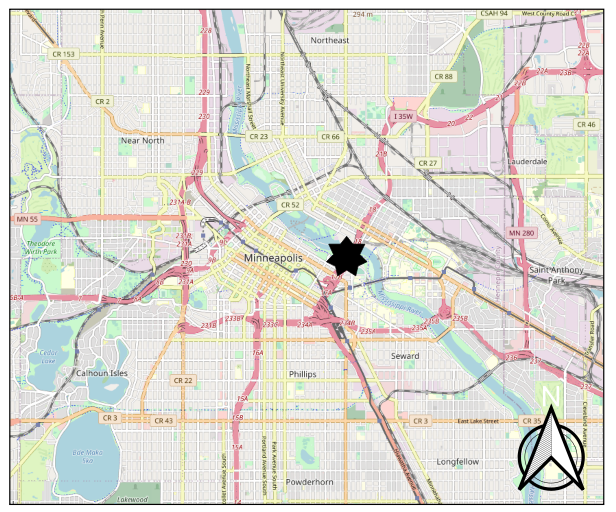
\includegraphics[width=0.75\linewidth]{figures/chapter2/I-35W.png}

}

\caption{Approximate location of the I-35W bridge collapse.}\label{fig:i35}
\end{figure}

\citet{zhu2010} conducted a travel survey that provided a more in-depth
analysis of important data
and traffic changes surrounding the I-35W bridge collapse in 2007. The
article used a methodology
that attempted to identify mode-choice and other behavioral changes of
survey respondents. The
authors analyzed data looking for variations in ADT, as well as origin-destination (OD) matrices.
Importantly, they analyzed loop detector data, bus ridership statistics, and survey response data in their work. The
authors conducted a regression analysis of the collected data,
which indicated that drivers are reluctant to make mode choice changes,
rarely doing so in the real world. This is
likely due to finances, time, or perceived difficulty of
navigating a new mode of
transport. At the same time, some drivers easily change destinations or routes when faced
with increased travel
times.

\citet{levinson2010} explored traffic behavior and changes in the wake of
major network
disruptions such as those that occurred in Minnesota. The authors identified
unique behavior, post
disaster, using GPS tracking data, survey data from the post disaster
phase, and other aggregate
data from surrounding freeways and traffic devices. These data were
analyzed to track
changes in ADT over bridges and alternate routes in the area after the
disaster as well as
after mitigation was complete. The authors provided increased
understanding about how a
network's operability changes in a post-crisis environment.

\citet{xie2011} attempted to determine economic costs in the form of
increased travel time
of the 2007 I-35W bridge collapse using a scaled-down travel demand model.
The authors used a
simplified version of the SONG 2.0 travel demand model that had been
developed for the Twin
Cities area to determine vehicle hours traveled (VHT) and vehicle
kilometers traveled (VKT). They
also calculated the accessibility for each zone, from jobs to workers, and
from workers to jobs, of
the network using employment, residency, and transportation cost data.
Using this simplified
gravity-based travel demand model, the authors estimated that the bridge collapse cost the Twin
Cities approximately
\$75,000 per day in increased travel times. Interestingly, they are able to
show that accessibility between workers and jobs was heavily affected by the
loss of the bridge. The ease with which road users can access locations around the region
experienced a dramatic decrease on the crippled network when compared to the whole, unbroken network.

\subsection{I-85/Piedmont Road Bridge Fire}

In Atlanta, Georgia, a section of bridge along I-85 near Piedmont Road collapsed due to a
massive fire under the bridge
on March 30, 2017. The fire grew
quickly because of
improperly stored construction materials under the bridge. The approximate
location of the bridge
collapse caused by the fire can be seen in Figure \ref{fig:i85}; the damaged link was
at a critical point
downstream of a merge point between two expressway facilities (GA-400 and
I-85) bringing commuter
traffic in from the suburbs of northern Fulton and Gwinnett Counties.

\begin{figure}
\begin{center}

{\centering 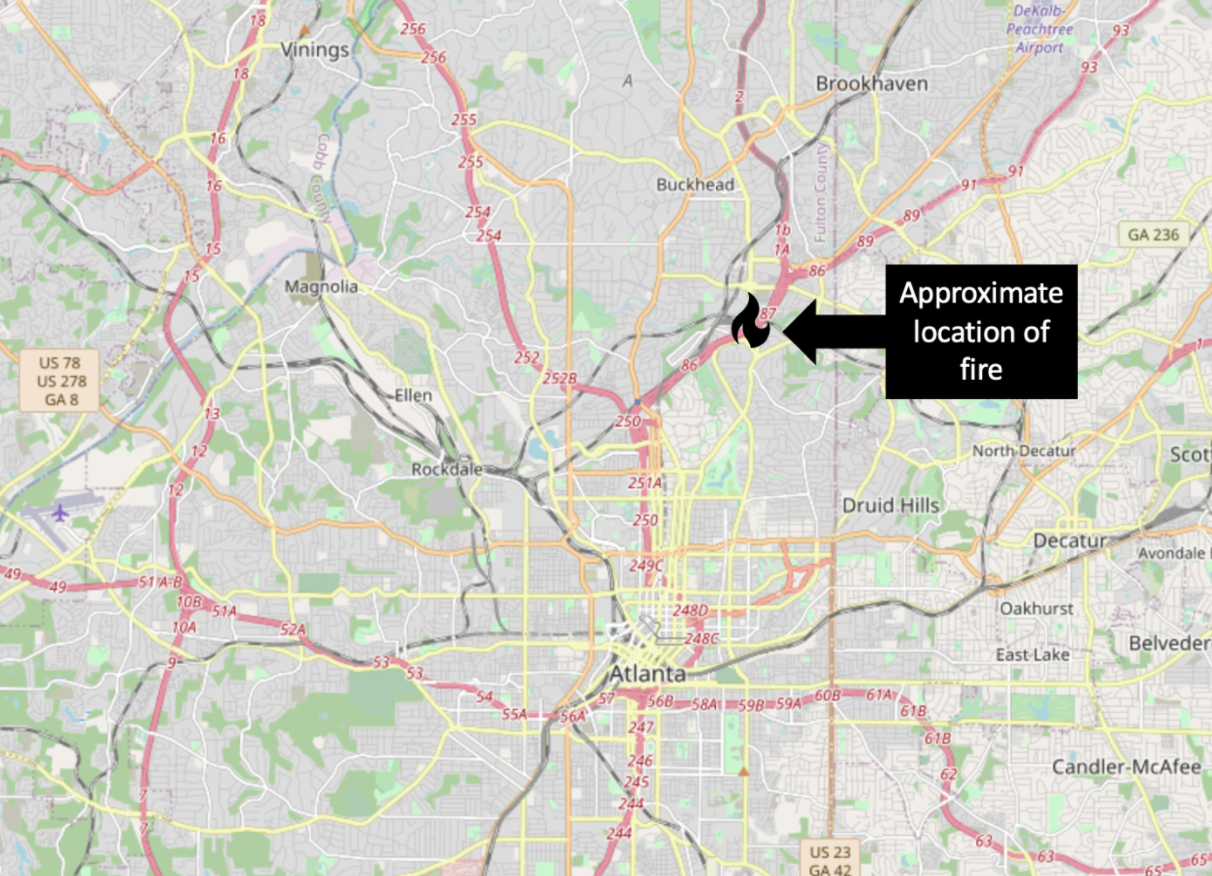
\includegraphics[width=0.75\linewidth]{figures/chapter2/I-85.png}}

\caption{Approximate location of the I-85/Piedmont Road bridge fire.}\label{fig:i85}

\end{center}
\end{figure}

The section of I-85 that was closed impacted a large, upper income
demographic in the greater
Atlanta area who commuted across the bridge.
As a result, the Georgia Department of Transportation (GDOT) along with
the Governor created a
\$3.1 million incentive program to help motivate project completion ahead
of schedule. The bridge
was originally scheduled to be closed for a period of 10 weeks, however, it re-
opened after just 6
weeks, with construction being completed a month ahead of schedule. The
accelerated finishing
date was estimated to have saved approximately \$27 million in user and
travel time costs
\citep{GDOT2017}. GDOT’s efforts to reconstruct the bridge and quickly reopen the highway after the
bridge collapse and immediate highway closure aided in abating negative user costs (or dis-benefit) due to significant travel
time delays that surfaced (in a post-disaster environment)
due to changes in route choice and assignment.

As a result of the fire, the highway, which had an ADT of 243,000,
was closed in both directions for a period of about six weeks. This
closure led to a sudden 30\%
increase in traffic volumes across the entire downtown network, with
notable increased congestion on side
streets \citep{hamedi2018}. Additionally, the Metropolitan Atlanta Rapid
Transit Authority
(MARTA) experienced a 20\% increase in ridership, likely because many
commuters made mode choice
and route changes. To mitigate this, headways between buses and trains
were decreased to allow
greater passenger volume. MARTA was also able to extend service capacity by about 20\%, adding 142,000 rail miles, 1,100
train hours, 8,202 bus
miles, 512 bus hours, and 2,463 parking spaces in park and ride lots to
help further mitigate the sudden increase in ridership \citep{marta2017, marta2018}. It is likely that MARTA’s efforts
to mitigate the rapid increase in passenger
volumes greatly reduced any negative effects of the bridge
fire on transit services, and helped alleviate other congestion generated by the disaster.

\section{Attempts to Evaluate Systemic Resiliency}

Real world events do occur; however, and it is important for researchers to
base efforts on both theoretical scenarios, and on actual events.
Thus, a number of researchers have conducted studies where real
or fabricated transportation networks are constructed, damaged or degraded, and
then the change to network metrics is evaluated. All of this is done to measure
network performance without
an actual disaster occurring beforehand.

\citet{berdica2002}
attempted
to identify, define and conceptualize vulnerability by envisioning
analyses conducted with
several vulnerability performance measures, including travel time, delay,
congestion,
serviceability and accessibility. Here, Berdica defined accessibility as
the ability for users to
travel between OD pairs for any number of reasons. She
then used the performance
measures to define vulnerability as the level of reduced accessibility due
to unfavorable
operating conditions on the network. In particular, Berdica identified a
need for further
research toward developing a framework capable of investigating or measuring
the overall systemic resiliency of transportation
networks.

In the following section, the work of several researchers who have attempted to develop
a framework capable of investigating or measuring the overall systemic resiliency
of transportation networks will be examined. Many of the researchers use different
methods to measure network performance while a network is operating under some kind of duress,
and a consolidation of this
discussion is summarized
in Table \ref{tab:authortable}. The measures can be consolidated into three
basic species of study:

\begin{enumerate}
	\item {Network connectivity}: How does damage to a network
	diminish the connectivity
between network nodes?
	\item {Travel Time analysis}: How much do shortest path travel
	times between origins
and destinations increase on a damaged network?
	\item {Accessibility analysis}: How easily can the population
	using the damaged
network complete their daily activities? This in turn can be evaluated in a number of ways as explained by \citet{dong2006}.
\end{enumerate}

The following sections discuss relevant studies in each group; Table
\ref{tab:authortable} consolidates these studies by year and labels them
with
an applicable group.

\begin{table}

\caption{\label{tab:authortable}Attempts to Evaluate Systemic Resiliency}
\centering
\begin{tabular}[t]{lll}
\toprule
Author & Year & Performance Metric\\
\midrule
Geurs and Van Wee & 2004 & Accessibility (isochrone, gravity, logsum)\\
Dong et al. & 2006 & Accessibility\\
Koppelman and Bhat & 2006 & Accessibility (isochrone, gravity, logsum)\\
Abdel-Rahim et al. & 2007 & Network Connectivity\\
Berdica and Mattson & 2007 & Network Connectivity\\
\addlinespace
Taylor & 2008 & Accessibility (logsum)\\
Peeta et al. & 2010 & Travel time and cost\\
Geurs et al. & 2010 & Accessibility (logsum)\\
Jenelius & 2010 & Network Connectivity\\
Zhu et al. & 2010a & Travel time and cost\\
\addlinespace
Zhu et al. & 2010b & Travel time and cost\\
Agarwal et al. & 2011 & Network Connectivity\\
Ip and Wang & 2011 & Network Connectivity\\
Serulle et al. & 2011 & Travel time and cost\\
Ibrahim et al. & 2011 & Travel time and cost\\
\addlinespace
Xie and Levinson & 2011 & Accessibility (isochrone)\\
He and Liu & 2012 & Travel time and cost\\
Masiero and Maggi & 2012 & Accessibility \\
Omer et al. & 2013 & Travel time and cost\\
Osei-Asamoah and Lownes & 2014 & Network connectivity\\
\addlinespace
Guze & 2014 & Network connectivity\\
Zhang et al. & 2015 & Network connectivity\\
Jaller et al. & 2015 & Travel time and cost\\
Xiangdong et al. & 2015 & Network connectivity\\
Nassir et al. & 2016 & Accessibility \\
\addlinespace
Winkler & 2016 & Accessibility (gravity)\\
Ganin et al. & 2017 & Accessibility (gravity)\\
Vodák et al. & 2019 & Network connectivity\\
\bottomrule
\end{tabular}
\end{table}

\subsection{Network Connectivity}

Graph theory is the mathematical study of networks of nodes connected by
edges (links). Concepts closely related to graph theory, such as network
vulnerability and network connectivity, have been studied by researchers.
In these studies, researchers tend to define
critical links as those
that are well connected to many other nodes (directly or indirectly), or as links
whose loss easily isolates a
number of nodes from the rest of the network \citep{west2001}.

\citet{abdel2007} developed a multi-layered graph approach to examine the resiliency
of the traffic
signal control system in Boise, Idaho. The researchers determined which
traffic signals would be isolated by a failure to a particular power
substation,
and consequentially the percent of travel paths that would experience
diminished
levels of service. The research highlighted the degree to which interrelated
infrastructure systems -- power, telecommunications, and transportation --
depend on each other, though the researchers did not attempt to look at the
connective resiliency of the transportation network directly.

\citet{agarwal2011} presented a method to represent a transportation network
as a
hierarchical, or cluster graph, that can be analyzed more directly for
vulnerabilities. Clusters are formed as groups of links and nodes become
isolated from each other. These clusters of links and nodes are then grouped
together more tightly by including nearby clusters, which creates a
``zoomed out'' or less complex model where small clusters begin to act as nodes connected by links.
In the study, links in the system are damaged, and the resulting
connectedness of the network is evaluated. One scenario of importance
noted by the authors, however, is that a maximal failure consideration where a
node
is entirely isolated from the network is unlikely in a real-world network
with
multiple paths of connectivity. The authors discussed the importance of
having damaged networks with high levels of functionality.

\citet{vodak2019}
on the other hand, developed an approach to identify
critical links in a network by searching for the shortest independent
loops in the network. An independent loop is essentially a way to travel
between an origin and a destination over any number of alternative routes.
The algorithm progressively damaged one or more links
between iterations to determine if nodes become isolated, or cut off from
the
network. If a node becomes easily isolated or has a higher likelihood of
becoming isolated, then there is a higher degree of vulnerability present
in the
network. This method can both identify critical links in individual
networks and provide a means to quantitatively compare networks.

\citet{ip2011} addressed this shortcoming through the concept of
{friability}, or
the reduction of capacity caused by removing a link or node, in order to
determine criticality of individual links. The methodology relied on the
ability
to determine the weighted sum of the resilience of all nodes based on the
weighted average of connectedness with other city nodes in the network. The
authors determined that the recovery of transportability between two cities
largely depends on redundant links between nodes. The authors also commented
that
most traffic managers are more concerned with the friability of single
links
rather than the friability of multiple links or an entire system. This suggests
that planners and managers may not consider the importance of
understanding the impacts of widespread, all-inclusive disaster scenarios.

\citet{guze2014} conducted a review of the known uses of graph theory
(a possible application of resiliency) before
reviewing several
other multi-criteria optimization methods.
Graph theory is the study of pairwise objects, and is
useful for identifying
shortest path, network connectivity, and other methods of network
optimization \citet{west2001}. Graph theory
supports the idea of resilience through recovery as well as operability through crisis discussed in
Section \ref{sec:ch2overview},
because of how it
represents networks with links and nodes, and the theory's ability to identify next
shortest paths in the
case of disaster. Guze’s methodology
involved an
analysis of the knapsack problem which is a combinatorial optimization problem.
Specifically, Guze focused on flow
theory in transportation
systems and identifying a method to find the best graph solution. Guze’s
greatest contribution to transportation research
at the time, was a simplified method
for determining shortest path route options on simple networks.

\citet{osei2014} adopted a network analysis methodology that is able to
analyze
resilience of transportation networks. In this
article, the authors evaluated resilience by comparing the biological
network of a common mold
with a rail network. The network for both the mold and the railway are
complexly connected. The ``giant'' component, a construct of a graph representing its connectivity, is given by:

\begin{equation}
	\Phi = \frac{E'}{ E}
\end{equation}

\noindent where $\Phi$ represents the giant component, $E$ represents the
level of connectivity before the network is damaged, and $E'$ represents the
level of network connectivity after the network is damaged. After the giant component
is found, network efficiency is determined using the
shortest path available. By combining both the ratio of link connections and
network efficiency, the authors draw comparisons between two
complex networks. Ultimately, the authors concluded that a denser, more highly
interconnected network would perform better when a link is cut due to a larger giant component value.

\citet{zhang2015} investigated the role of network topology, or the physical
layout of the network in a geographic location.
The authors provided several examples of network topology types including
hub and spoke, grid, and
ring networks. After computing resilience indexes, or general resilience
levels of each type of
network topology, the authors determined that metrics such as throughput,
connectivity and average
reciprocal distance increased with greater lineage, however these same measures decreased as
networks became
more widespread. This is likely because larger networks typically have fewer, less dense node
connections, and
therefore are less redundant.

Each of the graph theoretical approaches discussed in this section tend to break
down in efficiency or connectivity as networks become larger. Real-world
networks are typically extremely large, with nodes and links numbering in the
hundreds, if not thousands. Thus, the connectivity of a node may be high though
connectivity may not be an accurate representation of a node's importance.

\subsection{Changes in Travel Time}

Highway system network failures --- in most imaginable cases --- degrade
the
shortest or least cost path, but typically do not eliminate all paths.
The degree
to which travel time increases when a particular link is damaged, or a node
becomes isolated, could
provide an estimate of the criticality of that link or node. If a link or node
becomes completely isolated, the travel time to that node or link would
increase indefinitely. Thus, ensuring total isolation of a node or link does
not occur becomes highly important to network resiliency in terms of graph theory.

\citet{Berdica2007} attempted to examine what the effects of road
degradation on Stockholm's transportation network would be if one or more
chokepoints were to become damaged or all-together inundated. The authors
sought to determine how interruptions affect the system, and how overall
system performance was affected. Users in this method were only given the
choice of an alternate route, and the authors acknowledge that this is not
entirely reasonable in a real world situation. This method purely attempted
to quantify delay experienced by users compared to the original
equilibrium state, but does make an attempt to determine a monetary value
associated with closure or degradation.

\citet{Jenelius2010} attempted to examine the importance of a link that
becomes critical only after partial network degradation, or redundancy
importance. This measure is primarily flow-based. In the presented context,
flow-based measures aimed to analyze and evaluate changes in the number of
vehicles that used a route given adverse circumstances on the network.

\citet{peeta2010} constructed a model to efficiently allocate
highway maintenance and emergency response resources at locations throughout a
network. Each link in the sample network was
assigned a specific failure probability based on resource allocation;
the model evaluated the increase in travel time resulting from a broken
link. The authors applied a Monte Carlo simulation of multiple scenarios,
which revealed resource allocation plans with the least network degradation,
and thus which links were most critical to the network's operations.

\citet{serulle2011} clarified variables related to resiliency
of transportation networks including average delay and transport cost,
adjusting interactions,
and increasing metric transparency. The authors employed a methodology
capable of quantifying
resiliency using a fuzzy interference approach – an approach meant to use
imprecise or vague data
– that relates physical and performance characteristics. The employed approach
is able to determine a
resiliency index that supports comparative and sensitivity analyses.
Accessibility data, including
available road capacity, road density, alternate route proximity, average
delay, transport cost,
and average speed reduction, are analyzed for importance to the integrity
of the network.

\citet{ibrahim2011} provided an approach for determining
vulnerability of infrastructure by estimating the cost of single link
failure based on the increase in shortest path travel time due to
increased congestion
levels. The authors proposed a hybrid heuristic approach that calculates the
traditional user-equilibrium assignment for finding the first set of
costs, and
then fixes those costs for all following iterations to determine the
effects of
failure on overall travel time of the system.

\citet{omer2013} proposed a methodology for assessing the resiliency of
physical infrastructure
during disruptions. To do this, the authors used a network model to build
an origin-destination
matrix which allows initial network loading and analysis. Omer’s model used
several metrics, but
the main metric used to determine resiliency is the difference in travel
time between a disturbed
and undisturbed network. Omer’s framework is applied to an actual network
between New York City
and Boston for analysis. Changes in demand, travel time, mode choice and
route choice are tracked
for analysis. Omer’s framework supports operability of transportation
networks (as seen in Section \ref{sec:ch2overview} due to the way it
analyzes networks experiencing suboptimal circumstances. The Omers's work
identified key
parameters that should be measured to assess resiliency during disruptive
events.

\citet{jaller2015} sought to identify critical infrastructure based on
increased travel time or
reduced capacity due to disaster. The proposed methodology utilized user-
equilibrium to determine
proper initial network loading. Then the shortest path between one origin
and one destination
could be identified. To implement damage to the network, a link was cut, and
then the next shortest
path was found. This process is followed for all links in the system in
order to determine a sense
of the criticality of each link to network resiliency. The analysis is
carried out for each OD
pair, and the nodes which experience the greatest change in travel time are determined to
be the most critical.
Jaller’s methodology allowed traffic managers to identify critical paths
for mitigation purposes
before the occurrence of disaster through careful analysis.

A primary limitation with increased travel time methodologies is that they
ignore other possible ways a population might adapt its travel to a
damaged
network. Some people may choose other modes or destinations, and it is
possible
that some previously occurring trips might be canceled entirely. It may also be
prudent to consider how access changes, and evaluate changes in user choice
based purely upon accessibility.

\subsection{Changes in Accessibility}
\label{sec:cacc}
In a travel modeling context, {accessibility} refers to the ease
with which
individuals can reach the destinations that matter to them; this is an
abstract
idea but one that has been quantified in numerous ways. \citet{dong2006}
provide a
helpful framework for understanding various quantitative definitions of
accessibility that we will simplify here. The most elementary definition of
accessibility is whether a destination is within an isochrone, or
destinations accessible within the same distance or time interval from an origin.
This measure is often represented as a count (e.g., the number
of jobs
reachable from a particular location within 30 minutes travel time by a
particular mode). Mathematically, accessibility is defined as:

\begin{equation}
A_i = \sum_{j} X_j I_{ij}; I_{ij} = \begin{cases}  1 \text{ if } d_{ij}
\leq D\\
0 \text{ if } d_{ij} > D \end{cases}
	\label{eqn:isochrone}
\end{equation}

\noindent where the accessibility \(A\) at point \(i\) is the sum of the all the
destinations \(X\) at other points \(j\). \(I_{ij}\) is an indicator
function equal to
zero if the distance between the points $d_{ij}$ is less than some asserted
threshold (e.g., 30 minutes of travel time). By relaxing the
assumption of a
binary isochrone and instead using the distance directly, we can derive part of the
so-called gravity model,

\begin{equation}
A_i = \sum_{j} X_j f(d_{ij})
  \label{eqn::gravity}
\end{equation}

\noindent where the function $f(d_{ij})$ is often a negative exponential with a
calibrated
impedance coefficient. An extension of the gravity model is to use the
logsum
term of a multinomial logit destination choice model,

\begin{equation}
A_i = ln\sum_{j} \beta_d(d_{ij}) + X_j\beta
  \label{eqn:logsum1}
\end{equation}

\noindent where the parameters $\beta$ are estimated from choice surveys or
calibrated to
observed data. The logsum term has numerous benefits outlined by
\citet{handy1997}
and \citet{geurs2004}; namely, the measure is based in actual choice
theory, and
can include multiple destination types and travel times by multiple
different modes.

\citet{geurs2004} provide a review of accessibility measures such as those
above, up to
2004 in a literature review done at the time. Of the papers they reviewed, \citet{vickerman1974}, \citet{ben1979}, \citet{geurs2001}, used isochrone type methods. \citet{stewart1947}, \citet{hansen1959}, \citet{ingram1971}, \citet{vickerman1974}, \citet{anas1983}, used gravity
style models, and \citet{neuburger1971}, \citet{leonardi1978}, \citet{williams1978}, \citet{koenig1980indicators}, \citet{anas1983}, \citet{ben1985discrete}, \citet{sweet1997aggregate}, \citet{niemeier1997accessibility}, \citet{handy1997}, \citet{levine1998rethinking}, \citet{miller1999measuring} used or
suggested logsums. These researchers highlight the importance of using person-based
measures such as logsums in
evaluating network vulnerability and resiliency.

\citet{taylor2008} applied logsum-derived accessibility analysis to
evaluate the consequences of a tunnel failure in Adelaide, Australia. An
accessibility framework capable of evaluating the change in accessibility
for a multimodal urban network was designed. The designed framework is
capable of determining the ability of an individual to access an activity.
Taylor's framework captured five types of choice, namely: activity, time period,
trip-base, location, and mode choice, with key features being activity
choice and trip-base (e.g., the origin point of a trip). Each of these choice
models use typical multinomial logit models (MNL), with the exception of
the mode choice model, which uses a nested MNL model. The main choice
considered in the framework is activity choice followed by trip choice.
Taylor's proposed framework has been applied to an existing activity based
choice model for the Adelaide region, however, the framework operates
independently from the parent model.

Using the developed framework, Taylor calculated an ``inclusive value'' (IV)
and ``consumer surplus'' (CS) value. Both the IV and CS values are vital to
determining the benefit or dis-benefit
associated with the change experienced by users in the individual model
scenarios considered.

Taylor's accessibility framework, applied as a separate or connected module to
the Adelaide model, estimates the IV and CS values using a logsum.
These values allowed Taylor to show that more disruption occurs near the
failed link than occurs farther away. Additionally, Taylor is able to show
that a greater cost (nearly 40 times greater) is experienced by those who
live in a TAZ near the link than by those who live in a TAZ located
farther away from the failed link. Taylor's framework primarily
investigated accessibility on a network for a large city,
but could easily be applied on a larger scale.

In the Adelaide model, Taylor breaks one link and
then calculates the difference in IV and CS values using:

	\begin{equation}
		E(CS) = \frac{1}{\alpha} \log (\sum_{j = 1}^{J} \exp (I_j)) + \beta
			\label{eqn:taylor}
	\end{equation}

\noindent where the \(\alpha\) represents the negative of the coefficient of time or cost from the utility function,
and \(\beta\) is an unknown constant that represents the difference between the actual value of CS and the estimated value.
The \(I_j\) term represents the observable attributes of the possible utility.

Taylor's research highlighted the possibility for a comprehensive model capable
of succinctly measuring the dis-benefit caused by a degraded network.
Taylor continued by stating that traffic network simulation models
could be considered for future research.  Four key needs for
future research specifically highlighted at the conclusion of Taylor's article include:

	\begin{enumerate}
		\item Efficient algorithm development
		\item Improved vulnerability metrics
		\item Use of network vulnerability indicators in studies of critical
		infrastructure and the implications of network degradation
		\item Improved techniques for identifying network weaknesses
	\end{enumerate}

\noindent Several other authors employed various types of logit models in their research,
or attempted to develop a methodology specifically for use in analyzing disrupted networks.

\citet{geurs2010} compared the benefits attributed to various climate
change-mitigation land use and transport policies under two different
evaluation metrics. The authors directly compared a “rule of half (RoH)”
calculation where the travel time reduction is distributed between existing
and new travelers on a route with a mode choice logsum derived from utility
theory. The authors argued that because the logsum is more comprehensive and
inclusive of the full changes to travel demand (capturing the total value of
the choice set), the additional benefits attributed to proposed projects are
both more realistic and more economically favorable to climate change
mitigation policies. They showed this by evaluating the accessibility and
travel time changes resulting from land use densification strategies in the
national travel demand model for the Netherlands.

\citet{Masiero2012} used logit-based calculations to determine the Value of
Time (VOT) associated with the closure of a road in terms of cost, time,
and punctuality for freight transport. In order to properly determine the
VOT of route closure, the authors also used a method discussed in
\citet{koppelman2006} which used model derived coefficients and values to
determine the cost of an alternative. The authors implemented their
model on a network consisting of a single travel corridor that has
experienced long (1 week to 2 months or more) closures in the past.

\citet{xiangdong2015} developed network-based measures and computational
methods to evaluate transportation network redundancy. This methodology used
two dimensions in the analysis: travel alternative diversity and network spare
capacity, meaning the number of effective connections available for each OD
pair and the congestion effect/choice behavior of travelers. To create the
analysis, the authors first constructed a sub-network which only looks at
efficient routes. Next, the method counted the number of efficient routes
from the origin to all nodes, and then estimates the multi-modal network
spare capacity. Each dimension helps evaluate the capacity of the network
based on different scenarios. Xiangdong's method supports operability
(seen in Section \ref{sec:ch2overview}) by evaluating the capacity of
transportation networks using altered or damaged networks.

\citet{Nassir2016} applied a nested logit model to examine a transit
network in Australia. The main contribution in \citet{Nassir2016} is an
improved methodology for calculating accessibility measures related to
transit, accomplished by developing a method to account for diversity
information. The authors did note, however, that this measure is best applied
to models with complex transit systems that serve large portions of the
community. One important observation, however, is that users did not always
choose the fastest route, nor did they always choose the route with the
highest utility. \citet{He2012} took another look at the after effects of
the I-35W bridge collapse previously discussed. A key contribution of
\citet{He2012} is that people often initially base route choice on what they
assume will be best based on past experience. So, over time, users
adjusted their route choice to an altered network. The true implication here
is that users did not automatically choose the best new route given an
altered network, rather, it takes users time to learn how the new network
functions.

\citet{winkler2016} proposed a travel demand model that is valid for all
networks,
especially those with more than one constraint.
Winkler’s methodology
utilized a
model that uses production, distribution, and mode choice as inputs. The
methodology shows that models can be used to help determine outputs for
multi-constraint MNLs. Logsums like Winkler’s
also allow for consumer surplus calculations,
or utility, to be estimated across the transportation network
being modeled.

\citet{ganin2017} attempted to investigate resiliency through a disruption
of 5\% of the roadways
in 40 urban networks within the United States. The employed methodology
determined that Salt Lake
City had the most resilient transportation network while Washington D.C.
had the least resilient.
This determination is based on a comparison of simple gravity models of the identified networks after links are
damaged versus before.
The authors worked three factors into each model, which account for
differences in car-
truck ratios, average speed, and average vehicle length. Using a gravity
model to determine commuting patterns, the authors were
able to estimate the average
annual delay per commuter. They used this to determine network efficiency.
\citet{ganin2017} noted that
traffic delay times (or the travel time caused by a closure) increased
significantly as road segments were broken.

\section{Summary}

The lessons learned from the events in Minneapolis and Atlanta demonstrate
that when
transportation networks are damaged or degraded by link failure, multiple
changes result. Traffic
diverts to other facilities and other modes, and some people make
fundamental changes to their
daily activity patterns, choosing new destinations or eliminating trips
entirely. Numerous other
researchers have identified methodologies to capture the effects, or at
least have made quality attempts to capture the costs of these
potential changes to accessibility in modeled crisis events. Some researchers
have even applied logit-based models to small scale activity-based models.
From this extensive review of existing literature, we are able to see that no
one has attempted evaluate the relative systemic
criticality of highway links on a statewide network using a logit-based model
sensitive to changes in route path, destination choice, and mode choice.

\chapter{Model Design and Implementation}
\label{chp:chapter3}
\graphicspath{{figures/}{figures/chapter3/}}

\section{Overview} \label{Overview}

The objective of this study is to evaluate the relative systemic
criticality of highway links on a statewide network using a logit-based model
sensitive to changes in route path, destination choice, and mode choice.

In this chapter, some of USTM's properties are described, and additional detail is give as to why
USTM is not entirely suitable for this study as presently constituted. A new
model framework designed to evaluate resilience using a logit-based choice model on
USTM's network is then presented. Implementation of this new model within the CUBE travel demand
modeling software is also described.

\section{Utah Statewide Travel Model} \label{Utah Statewide Travel Model}

UDOT manages an extensive highway
network consisting of interstate highways (I-15, I-80, I-70, and I-84),
intraurban expressways along the Wasatch Front, and rural highways throughout
the state. The rugged mountain and canyon topography places
severe constraints on possible redundant paths in the highway network outside and between urban areas. A
landslide or rock fall in any single canyon may isolate a community or force a
redirection of traffic that could be several hours longer than the preferred
route; understanding which of these many possible choke points is most
critical is a key and ongoing objective of the agency.

USTM is developed and maintained by
the travel demand modeling group at UDOT, and focuses exclusively on
long-distance trips. Within Utah, there are five travel
demand models developed for urban centers under the purview of  Metropolitan
Planning Organizations (MPOs). USTM incorporates these other models as inputs and covers
the rural areas lying outside of the MPO model regions. Consequently, USTM covers the
highway facilities across the entire state, and incorporates the MPO models
developed by the Wasatch Front Regional Council (WFRC), Mountainland
Association of Governments (MAG), Cache Metropolitan Planning Organization, and the Dixie Metropolitan Planning Organization. Additionally,
the Summit/Wasatch Travel Demand Model is incorporated into USTM \citep{udot2021}.
USTM as currently
constituted can be used for infrastructure planning purposes, but would be
inadequate to evaluate the systemic resiliency of the highway network given
the disparate methodologies of the MPO models incorporated. USTM can, however, provide the
following data elements:

\begin{description}
\def\labelenumi{\arabic{enumi}.}
\item
  [Highway Network] {including free flow and congested travel speeds,
  link length, link capacity estimates, etc.}
\item
  [Zonal Productions] {available for all zones by purpose,
  including those in the MPO region areas}
\item
  [Calibration Targets] {USTM base scenario estimates of mode split and
  trip length that could be used to calibrate the utility coefficients of a new model}
\end{description}

Each of the local travel demand models and USTM employ a gravity-based trip
distribution model. The gravity model assumes that trips between OD
pairs are proportional to total productions $P$ and
attractions $A$ throughout the state. That is, all productions will be
attracted to a location based on the size of a location (i.e., a location's
attractiveness) and the impedance (or friction) factor between the OD
pair. A mathematical representation of the gravity model is given by:
\begin{equation}
T_{ij}= \frac{P_i*(A_j F_{ij})}{\sum_{j\in J}(A_j F_{ij})}
 \label{eqn:gravity}
\end{equation}

\noindent where $T_{ij}$ represents the trips made between an origin $i$ and a
  destination $j$ among all destinations $J$, $P_i$ represents the productions at origin $i$, $A_j$ represents the attractions and destination $j$, and $F_{ij}$ is the impedance factor between an $OD$ pair.
The friction factor (also known as the impedance, or resistance to movement) between two
zones can be represented in a number of ways, such as with a negative
exponential function:
\begin{equation}
	F_{ij} = \alpha \exp(-\beta * d_{ij})
  \label{eqn:fricfac}
\end{equation}

\noindent where $d_{ij}$ is the distance or cost between zones $i$ and $j$, and $\alpha$
and $\beta$ are calibrated parameters. In the gravity model, as the distance
between an OD pair increases, users become less likely to make trips between
that OD pair.

A primary weakness of gravity-based distribution models is their inability to
consider multimodal impedances or other attributes of a destination other than
a destination's size (as represented by $A_j$ in Equation \ref{eqn:gravity}). The
impedance factor in Equation \ref{eqn:fricfac} asks an implicit question with its
distance or cost variable $d_{ij}$: which mode is used for the trip? In almost
all cases, automobile distances or costs are asserted as the only option, but if a
destination happens to be close by rail and far by highway, the gravity model
will not be able to incorporate this unless a mode split function is carried out first.

Alternatively to gravity models, logit-based models are becoming
increasingly more popular for trip distribution. Logit-based destination choice models improve model
sensitivity compared with gravity models, and are advantageous because
they possess an increased ability to introduce additional variables and reflect
other statistical assumptions into a model \citep{tfr2021}. A typical choice
model is made up of a combination of utility and probability values in the
following equations:

\begin{equation}
\mathcal{P}_{ij} = \frac{e^{u_{ij}}}{\sum_{j\in J}e^{u_{ij}}}
  \label{eqn:probability}
\end{equation}

\noindent where $\mathcal{P}_{ij}$ represents the probability of trips made between an
origin \(i\) and a destination \(j\) among all destinations $J$, and \(u\) represents the utility.
The log of the sum in the denominator of this probability --- called the logsum --- captures the total value of the all options in the choice set, and can be interpreted as the
benefit --- or dis-benefit --- experienced by users in a choice model \citep{williams1974},
\begin{equation}
 Logsum_{i} = \ln\sum_{j\in J}\exp(f(\beta, u_{ij}, A_j, \gamma, t_{ij}))
  \label{eqn:logsum}
\end{equation}
Where $\beta$ represents a mode choice coefficient, $u_{ij}$ represents the utility,
$A_j$ represents the attraction at zone $j$, $\gamma$ represents
a DC parameter, and $t_{ij}$ represents the travel time between an OD pair.

The ability to incorporate multiple types of data, as in Equation \ref{eqn:logsum}, as well as improved methods
for determining trip distribution, mode choice, and destination choice all allow
logit-based models to add an additional layer of sensitivity into estimations of
trips between OD pairs on a road network. Consequently, logit-based travel
demand models are better equipped to estimate the choice-based effects caused
by major changes to a road network, such as link loss or major link degradation
caused by adverse natural or man-made events.

Destination choice models explicitly consider multimodal accessibility, such as accessibility by automobile,
non-motorized trip, or transit. The ability to consider accessibility from a
multimodal perspective gives a user the ability to choose the location of
their destination based on a variety of factors including mode accessibility
(i.e. ease of access to a mode of transport). The information
derived from the socioeconomic data primarily comprises the size term, which
is a measure of the appeal or attractiveness of one destination when compared with
another destination. The DC size term is discussed in further detail in
Section \ref{sec:dc}.

A critical feature of logit-based choice models – described briefly in Section
\ref{sec:cacc} – is that they are more versatile than traditional modeling
methods, with the ability to incorporate different types of data --- \textit{and}
account for user choice. Additionally, logit-based choice models are better
able to measure the changes in accessibility of a destination due to network
changes than other models because of their adaptive nature. As such, logit-based
models are typically used in new or more advanced travel models.

Logit-based destination choice models are becoming increasingly common in four-
step and other modern travel models. However, no logit-based destination
choice models have been implemented within an MPO model in Utah or within
USTM except for some home-based work trips in the WFRC/MAG model. As a result,
the local MPO models, and therefore USTM, are not sufficient to analyze
accessibility on their own as proposed by this thesis. Therefore, a new
standalone model must be developed to examine choice-based resiliency in Utah.

\section{Model Design} \label{Model Design}

  \begin{figure}
    \centering
  {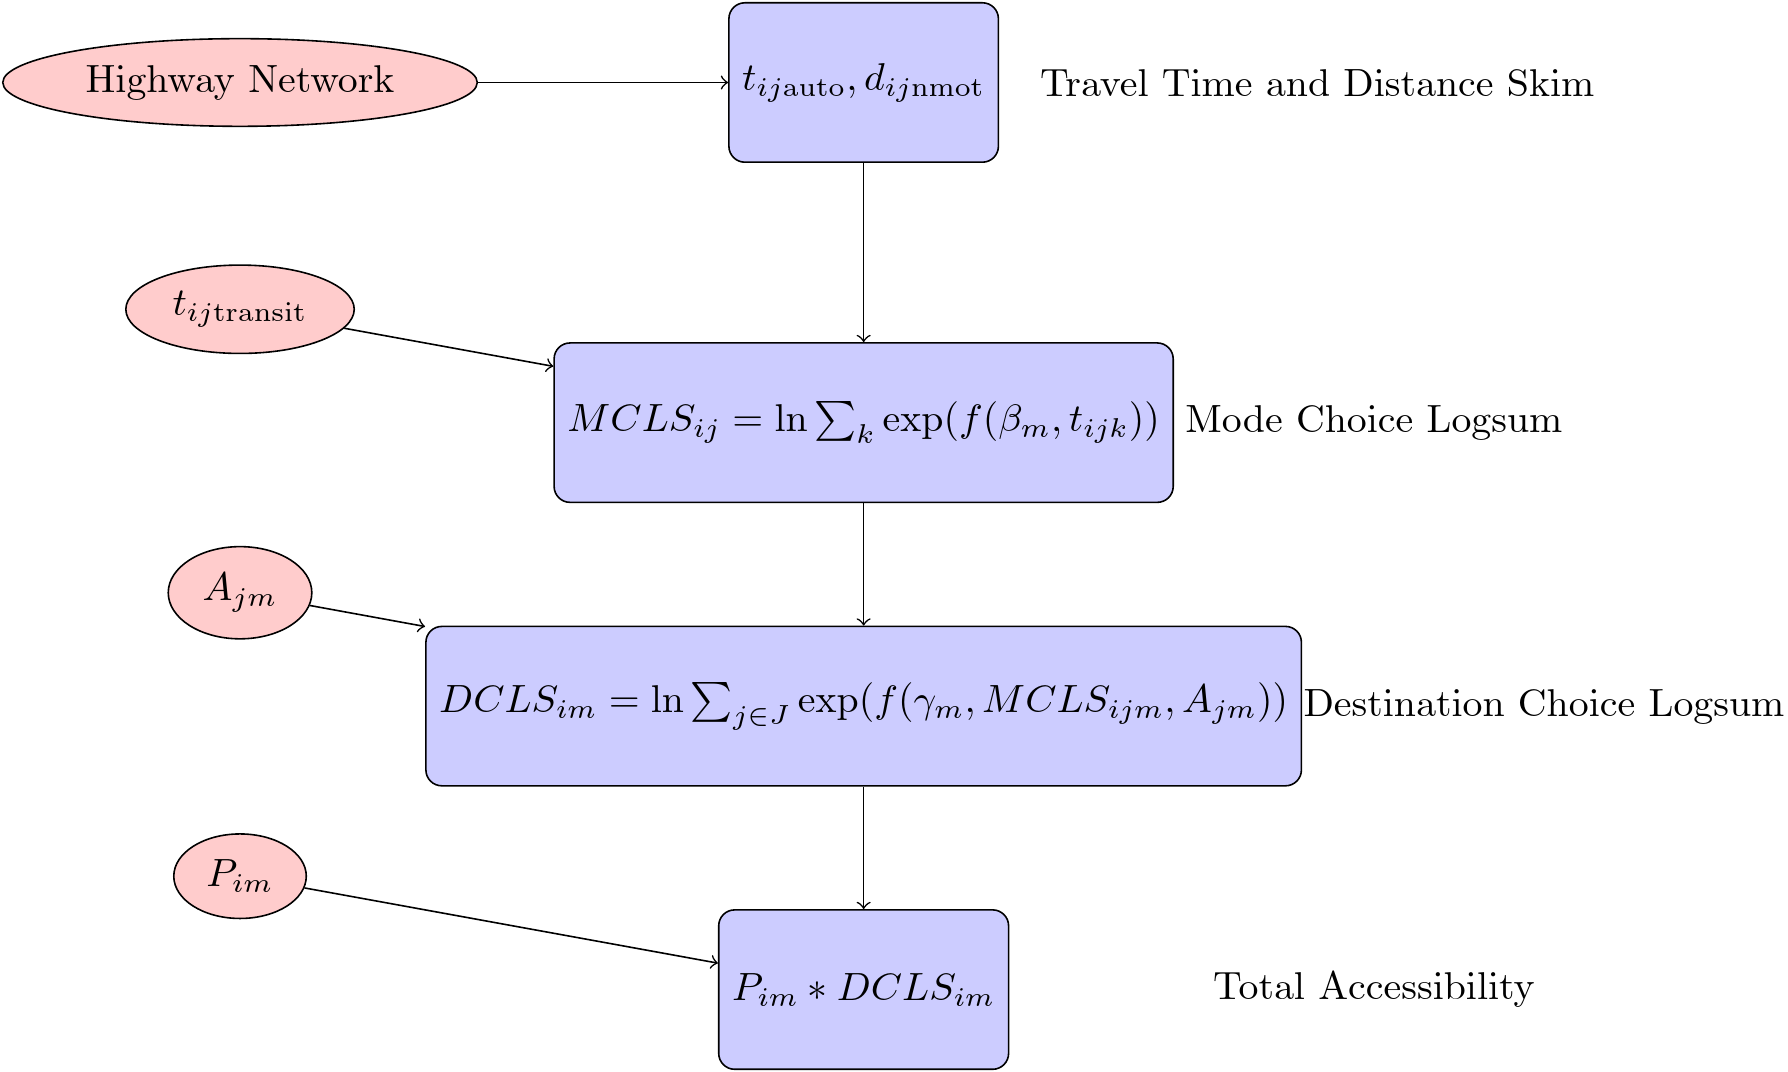
\includegraphics[width=0.75\linewidth]{figures/chapter3/framework.png}}
  \caption{Model framework.}\label{fig:framework}

  \end{figure}

An initial framework was developed to model the impact of link loss on the
USTM network. The model framework used to create the presented model
consists of the following steps:
\begin{description}
	\item [Skim Network] {In this step, the model determines the shortest
  path by AM peak travel time on the USTM network between each origin and
  destination. The model also determines the distance of the shortest time
  path. Transit times are given by an external data source.}
	\item [Mode Choice (MC) Logsum] {The MC logsum is a function of
  the travel impedances and serves as an impedance term in the destination
  choice model. The MC logsum contains utility functions that
  determine the probability and logsum associated with travel between each OD
  pair. The MC model also contains constants and coefficients that can
  be used to calibrate and adjust the utility equations, determining the mode
  choice probabilities.}
	\item [Destination Choice (DC) Logsum] {The destination choice logsum
  is a function of the travel impedances (represented by the MC logsum)
  and the attraction size term of each destination zone. This is the key
  evaluation metric of the model. The attraction size term is determined
  using socioeconomic data for each destination zone given by USTM.}
\end{description}
The model framework as used is presented in Figure \ref{fig:framework}, where
inputs are denoted with red ovals, and functions are denoted with purple rectangles.
The model framework is designed to capture the utility-based accessibility for
a particular origin zone \(i\) and trip purpose \(m\). The trip purposes considered
in the model include Home-based work (HBW), Home-based other (HBO),
and non-home based (NHB) trips. Other trips purposes, such as recreation (REC) trips and
Freight trips were not included because they either have fixed OD pairs, or do not generate a significant number of trips.
The model begins with a
travel time skim procedure, to determine the congested travel time from zone
\(i\) to zone \(j\) by auto (i.e., \(t_{ijauto}\)), as well as the shortest network distance (i.e., \(d_{ijnmot}\)) for non
motorized modes using the USTM network. The transit travel time skim is fixed, assuming that transit
infrastructure would not be affected by changes to the highway network, thus \(t_{ijtransit}\) is held fixed.
Throughout this section, acronyms from the model framework will be described and lower-cased index variables \(k\) belong to a set of
all indices described by the corresponding capital letter \(K\).

With the travel time \(t_{ijk}\) and distance for all modes \(k \in K\), the
model computes MC utility values. The multinomial logit MC
model describes the probability of a person at origin \(i\) choosing mode \(k\)
for a trip to destination \(j\):
\begin{equation}
\mathcal{P}_{ijm}(k) = \frac{\exp(f(\beta_m * t_{ijk}))}
{\sum_{K}\exp(f(\beta_m * t_{ijk}))}
  \label{eq:mcp}
\end{equation}

\noindent The log of the denominator of the this equation is called the
MC logsum, \(MCLS_{ijm}\) or \(MCLS\) and is a measure of the travel cost by
all modes, $k$, weighted by MC utility parameters \(\beta\) that may vary by
trip purpose $m$. The parameter values are described in greater detail in
Table \ref{tab:coeffs}.

The \(MCLS\) is then used as a travel impedance term in the multinomial
logit
destination choice model, where the probability of a person at origin \(i\)
choosing destination \(j \in J\) is
\begin{equation}
\mathcal{P}_{im}(j) = \frac{\exp(f(\gamma_m, MCLS_{ijm}, A_{jm}))}
{\sum_{J}\exp(f(\gamma, MCLS_{ijm}, A_j))}
  \label{eq:dcp}
\end{equation}

\noindent where \(A_j\) is the attractiveness --- represented in terms of
socioeconomic activity --- of zone \(j\). As with MC, the log of the
denominator of this model is the
destination choice logsum, \(DCLS_{im}\) or \(DCLS\). This quantity represents the value of access to
all destinations
by all modes of travel, and varies by trip purpose.

The \(DCLS\) measure is relative, but can be compared across
scenarios. The difference between the measures of two scenarios,
\begin{equation}
\Delta_{im} = {DCLS_{im}}^{\mathrm{Base}} - {DCLS_{im}}^{\mathrm{Scenario}}
  \label{eq:deltas}
\end{equation}

 \noindent provides an estimate of the accessibility lost when
 \(t_{ij\mathrm{auto}}\)
changes due to a damaged highway link. This accessibility change is \emph{per
trip},
meaning that the total lost accessibility is \(P_{im} * \Delta_{DCLS}\) where
\(P\) is
the number of trip productions at zone \(i\) for purpose \(k\). This measure is
given in units of dimensionless utility, but the MC cost coefficient
\(\beta\) provides a conversion factor between utility and cost. The total
financial
cost of a damaged link for the entire region for all trip purposes is:
\begin{equation}
\mathrm{Cost} = \sum_{I}\sum_{M} -1 / \beta_{\mathrm{cost},m} * P_{im}
\Delta_{im}
  \label{eq:totalcost}
\end{equation}

For comparison to a simpler resilience method that only includes the increased
travel time between an OD pair, we compute the change in travel
time, \(\Delta t_{ij}\), between two scenarios, and multiply the increase in
time by the number of trips in USTM. This is converted to a cost by a value of
time directly from USTM and UDOT \citep{UtahDepartmentofTransportation2020}. These
values can be seen in Table \ref{tab:VOT} at the end of this chapter. Converting to
a cost gives an estimate with units in
dollars per day. This conversion is accomplished with
\begin{equation}
\mathrm{Cost}' =  \sum_I \sum_J \sum_K VOT_{m} * T_{ijmk} t_{ijk}
  \label{eq:ttmethod}
\end{equation}

\noindent Deriving a simpler way to calculate resilience was necessary for two
reasons. First, data were not readily available for trips that do not have
flexible OD pairs, such as freight trips. Other purposes included in USTM,
such as recreation trips (REC) and trips that occur between external nodes
(i.e., inter-state trips that do not originate or terminate within the state),
make up very small percentage of total trips. Second, a method capable of
creating data that could be compared with the results of the presented logsum model
was needed. Calculating dis-benefit
based solely on increased travel time provides valuable insight and tools for
further analysis of the model results.

\section{Model Inputs}

Several inputs derived from various sources are needed for the presented model
to properly function. First, a highway network is needed which contains attribute
data needed to extract information about travel times and distances between
transportation analysis zones (TAZ). Additionally, a transit network is needed
because USTM does not explicitly consider transit. Non-motorized distances are
considered in the following sections.

\subsection{Transportation Network}

The presented logsum model requires an
understanding of the travel time and distance between zones by multiple modes, and how
these distances change when a link in the network is damaged or destroyed. To measure the
automobile, transit, and non-motorized trip times, initial data were needed for each trip mode.

The highway network is made up of both the urban and rural highway networks
for the whole state of Utah. The highway network contains many link- and
node-attribute data including street name, link distance, lanes, functional
classification, TAZ, county name,
as well as speed limits and travel time data for five different times of day.
Of particular interest from the available information was the \(AM\_TIME\) which
contains the travel time in minutes for the AM time period along a link and
the \(DISTANCE\), which contained the linear distance between nodes along a link.
The \(AM\_TIME\) was used to determine the travel time between an origin and
destination. The \(DISTANCE\) was used to measure the network distance between
the shortest OD pair based on AM travel time.

The highway skim module creates an output matrix (i.e., the highway skim) of travel
times and distances between OD pairs and must be created
before automobile (AUTO) and non-motorized (NMOT) trips can be incorporated
into the model. We used the \(AM\_TIME\) and \(DISTANCE\) variables available in
the highway network file to create a matrix of distances and shortest travel
times between all OD pairs in the USTM network. The output matrix forms the
basis for further analysis by providing the needed automobile and non-motorized
information for the other modules in the model.

\subsection{Transit Network}

Transit network resiliency is outside the scope of this project. Accordingly, transit services are fixed, meaning that changes to the
network do not influence transit availability on the network. However, transit
is an important mode to include in the model because of ample availability in Salt Lake City, and should be
considered in future model development if applicable for more robust analysis.
Among MPO models in Utah, only the model jointly operated by the WFRC and MAG model include a
substantive transit forecasting component. The transit travel time skim from the
WFRC/MAG model was used for the MC model in Equation \ref{eq:mcp};
the zonal travel time between the smaller WFRC/MAG model zones was averaged
to the larger USTM zones using a crosswalk, or matrix transformation function, and the minimum time among the several modes available
(commuter rail, light rail, bus rapid transit, local bus) was taken as the travel
time for a single transit mode in this implementation.

The non-motorized trip distances are held fixed, similarly to the transit distances. It was
determined that the longest distance a pedestrian would commute via a non-motorized
mode is 2.5 miles or less. The decision to hold non-motorized
trips constant was made for several reasons, mainly because pedestrians can usually
access routes that are not available to vehicles, such as neighborhood walkways/bikeways
or other shortcuts available only to pedestrians and cyclists. Additionally,
pedestrians are often also able to cut through or traverse the perimeter of an
area where a highway may be degraded or damaged. non-motorized trips also typically have
higher accessibility to smaller roads or side-streets that would not be included
with the USTM network.

\subsection{Socioeconomic Data}

The model uses socioeconomic data to estimate the trip productions at
each zone. The socioeconomic data, which is adapted from the Utah Travel Survey (UTS) conducted in 2013, contains TAZ related information such
as county name, total households, household population, total employment,
and a breakdown of employment by job category, among other data. This information is useful
when determining the DC attractions, or size term because they can be used to
describe population density of residential zones, or business density and type
of commercial zones in a network.

\section{Mode Choice Model}

The MC module calculates the MCLS between each OD pair in the
network for each trip purpose. The trip purposes considered in the model are HBW, HBO and NHB. The MC module includes the highway skim,
the transit skim, and the MC coefficients and constants as inputs.

The MC constants and coefficients used in the model were extracted
from USTM where possible, or adapted from the Roanoke (Virginia)
Valley Transportation Planning Organization (RVTPO) or SWIM models. The travel time represented with $t_{ij}$, travel cost
represented as a variable $C_{ij}$, walk distance (i.e., less than 1 mile) represented
as $d_{<1MILE}$, and walk distance (i.e., 1 mile or more) represented as $d_{>1MILE}$
are the coefficients for the
HBW, HBO,and NHB purposes. The MC coefficients were adapted
from USTM and supplemented with coefficients from the RVTPO travel model where USTM had gaps in the data \citep{rvtpoversion, swimversion}. This model was
selected as a source for these coefficients due to its simplicity and analogous data elements to the purpose of the presented model. The
values for each of the coefficients are in Table \ref{tab:coeffs}. The alternative-specific constants in the model were calibrated to regional MC
targets developed from the UTS using
methods described by \citet{koppelman2006}.

\begin{table}

\caption{\label{tab:coeffs}Choice Model Coefficients}
\centering
\begin{tabular}[t]{llrrr}
\toprule
 & Variable & HBW & HBO & NHB\\
\midrule
\addlinespace[0.3em]
\multicolumn{5}{l}{\textbf{Destination Choice}}\\
\hspace{1em} & $\gamma_{hh}$ Households & 0.0000 & 1.0187 & 0.2077\\
\hspace{1em} & $\gamma_{off}$ Office Employment & 0.4568 & 0.4032 & 0.2816\\
\hspace{1em} & $\gamma_{oth}$ Other Employment & 1.6827 & 0.4032 & 0.2816\\
\hspace{1em} & $\gamma_{ret}$ Retail Employment & 0.6087 & 3.8138 & 5.1186\\
\hspace{1em} & $\gamma_{MCLS}$ Mode Choice Logsum & 1 & 1 & 1\\
\hspace{1em} & $\kappa_1$ Distance & -0.0801 & -0.1728 & -0.1157\\
\hspace{1em} & $\kappa_2$ Distance squared & 0.0026 & 0.0034 & 0.0035\\
\hspace{1em} & $\kappa_3$ Distance cubed & 0.0000 & 0.0000 & 0.0000\\
\cmidrule{1-5}
\addlinespace[0.3em]
\multicolumn{5}{l}{\textbf{Mode Choice}}\\

\hspace{1em} & $\alpha_{TRANSIT}$ Transit constant & -0.3903 & -1.9811 & -2.2714\\
\hspace{1em} & $\alpha_{NMOT}$ Non-Motorized & -1.2258 & -0.3834 & -0.8655\\
\hspace{1em} & $\beta_{tt}$ Travel Time [minutes] & -0.0450 & -0.0350 & -0.0400\\
\hspace{1em} & $\beta_{cost}$ Travel Cost [dollars] & -0.0016 & -0.0016 & -0.0016\\
\hspace{1em} & $\beta_{d1}$ Walk Distance (less than 1 mile) [miles] & -0.0900 & -0.0700 & -0.0800\\
\hspace{1em} & $\beta_{d2}$ Walk Distance (1 mile or more) [miles] & -0.1350 & -0.1050 & -0.1200\\
\bottomrule
\end{tabular}
\begin{tablenotes}
      \small
      \item Note: The data in this table were extracted from the USTM, RVTPO, and SWIM models.
    \end{tablenotes}
\end{table}

The following are sample utility equations for each of the modes considered in
the model, where $\alpha$ denotes MC constants, $\beta$ denotes
MC coefficients, $\gamma$ denotes destination choice parameters, and
$C$ will denote other variables which are typically zonally related. Additionally,
the equations used to calculate the MCLS are shown:
\begin{align}
U_{{AUTO}_{ij}} &= \beta_{tt} * tt_{ij\mathrm{AUTO}} + \beta_{cost}* cost_{ij\mathrm{AUTO}} \\
U_{{TRANSIT}_{ij}} &= \alpha_{TRANSIT} + \beta_{tt} * tt_{ij} + \beta_{cost} * cost_{ij\mathrm{TRANSIT}} \\
U_{{NMOT}_{ij}} &= \alpha_{NMOT} + 20 * (\beta_{tt{}} * tt_{ij} + \beta_{cost} * cost_{ij\mathrm{NMOT}}) \\
Logsum_{ijm} &= \ln(\sum_K \exp (U_{ijmk})) \label{eqn:lsum}
\end{align}

From the equations above, several aspects between the three MC utility equations are
apparent. First, the transit and $NMOT$ utility equations both have a constant, denoted by a $\alpha$,
included. The $AUTO$ equation does not have a constant because auto serves as the reference
alternative in the presented model. Second, both the $AUTO$ and $NMOT$ equations account for a
distance variable. Finally, each of the three utility equations account for travel time, either in the
form of an in-vehicle travel time coefficient, or another modified factor. The $NMOT$ utility
equation is not calculated using a specific coefficient for time. Instead, the $NMOT$ distances are
multiplied by an assumed walking speed of 20 minutes per mile. This is common practice in other
choice models for $NMOT$ trips. After the MC utilities were calculated, it was necessary to calculate the logsum for
each trip purpose \(m\), as seen in Equation \ref{eqn:lsum}.

\section{Destination Choice Model}
\label{sec:dc}
The DC module
includes the MCLS, the socioeconomic data extracted
from USTM, and DC parameters as inputs, all of which are needed to estimate the DC utility value.
The DC utility equation consists of three parts: a size term \(A_j\),
a travel impedance term (MCLS value), and a several distance and cubic
calibration polynomial coefficients and their corresponding values.

The terms in the DC utility equation follow the same conventions mentioned
previously, however, \(d_{ij}\) is used to represent the distance variable in the calibration polynomial:
\begin{equation}
\begin{aligned}
	U_{ijm} = \gamma_{MCLS} * MCLS_{ijm} + \log (A_{jm}) + f(d_{ij})
\label{eqn:dc}
\end{aligned}
\end{equation}

\noindent where $f(d_{ij})$ is a calibration function discussed later in this section.

Coefficients for the
size term and travel impedance terms were adapted from SWIM \citet{swimversion}
for all purposes except HBW. Instead, these coefficients were
adapted from the RVTPO model \citet{rvtpoversion}. This was done because SWIM
does not account for work trips in the same way as it does other trip purposes.
The distance polynomial coefficients were
calibrated to targets developed from UTS.

The MCLS value is applied to the DC model utility equation as the impedance
term, or a measure of
a user’s resistance to using the specified path or mode. This is like the
impedance factor in the
gravity model discussed in Section \ref{sec:cacc}. Feeding the MCLS value into
the DC module is what allows
users to choose a destination while considering accessibility from all modes. In these
equations, the log terms serve to create the logsum values needed to find
the DC logsum values later on.
The size term, which
will be discussed in greater detail later in this chapter, helps to determine
the attractiveness
of a destination zone compared to another destination. The cubic polynomial
terms serve as a
method to calibrate the DC module outputs and will also be discussed in
greater detail later in
this chapter.

The socioeconomic data is used in the DC model to compute the size term, or
the attractiveness of
a destination in the model. The size term is made up of statistical
data about a zone. The size term is
created using various DC parameters combined with corresponding socioeconomic data
to determine the size or attractiveness of a zone. The size term equation was partially
adapted from the Oregon Statewide Integration Model (SWIM) \citep{swimversion}.

This data was published in 2013 as part of the UTS and made available via
UDOT \citep{uts2013}.  The size term
equation can be seen below:
\begin{equation}
\begin{aligned}
	A_{jm} = \gamma_{m_{off}} * \mathrm{office}_j + \gamma_{m_{oth}} * \mathrm{other}_j + \gamma_{m_{hh}} * \mathrm{hh}_j + \gamma_{m_{ret}} * \mathrm{retail}_j
	\label{eqn:sizeterm}
\end{aligned}
\end{equation}

\noindent where each different zonal socioeconomic element in the UTS data influences
utility through a corresponding $\gamma$ parameter.

The DC logsums are calculated by summing the exponentiated values in each row in the DC utility matrix
together. The process used to accomplish this can be seen
in Equation \ref{eqn:dc}. The value of the DC logsum is the accessibility of
a zone based on the zone's size and distance by multi-modal travel impedance.


\section{Model Calibration and Validation}

Modeling efforts can produce a wide range of estimates, and it is important to
check that model outputs are estimating trips accurately according to available trip data.
To ensure the model was accurately reflecting trips by MC in the USTM model,
the presented model  must be
calibrated accordingly. To do this, target values were extracted from
USTM for each trip purpose.

\subsection{Trips by Purpose and Mode}

In order to calibrate the model, trip totals needed to be calculated by purpose
(\(T_{ijm}\)) and by mode (\(T_{ijmk}\)). To find the trips by purpose
(\(T_{ijm}\)), the probability of a trip occurring between an OD pair needed to
be determined. Likewise, to find the trips by purpose and mode (\(T_{ijkm}\)),
we multiplied the \(T_{ijm}\) by the MC probabilities calculated during the MC
module. A mathematical representation of this can be seen in the equations
below:

\begin{equation}
	T_{ijm} = P_{im} * \mathcal{P}_{ijm}
	\label{eqn:ij}
\end{equation}

\noindent Where $P_i$ is the productions at zone i, and,

\begin{equation}
	T_{ijkm} = T_{ijm} * \mathcal{P}_{ijk}
	\label{eqn:ijk}
\end{equation}

\noindent The ability to account for trips by purpose and by mode allows us to
determine information about how well the model is calibrated, and the utility
values can also be used to determine the logsum calculations, which are capable
of accounting for more than one type of data.


\subsection{Calibrating Choice Constants}

The utility functions in Equations \ref{eqn:dc} and \ref{eqn:sizeterm} contain
calibration constants which are adjusted to calibrate the model. Model
calibration is completed by iteratively adjusting the MC
constants and DC constants to match extracted target values. The nature
of the presented model causes the MC and DC portions to interact. As such,
the best method for calibration was to iteratively run the model, changing
the MC constants and DC parameters after each new iteration was complete.

To calibrate the MC constants, the alternative specific constants must be
adjusted so that the mode split target extracted from USTM closely matches the
model mode split values. A multinomial logit model will use alternative-
specific constants to match a particular sample share. By adjusting these
constants, it is possible to match a MC model to target values.
Figure \ref{fig:nhbmc} shows the target values for each mode represented as a
dotted line, and shows the change of the MC calibration constants
(and the target shares for each purpose) over the five iterations;
the first iterations moved the calibration the most, with some adjustment
over the following iterations. Overall the fit is fairly good.

  \begin{figure}
  {\centering 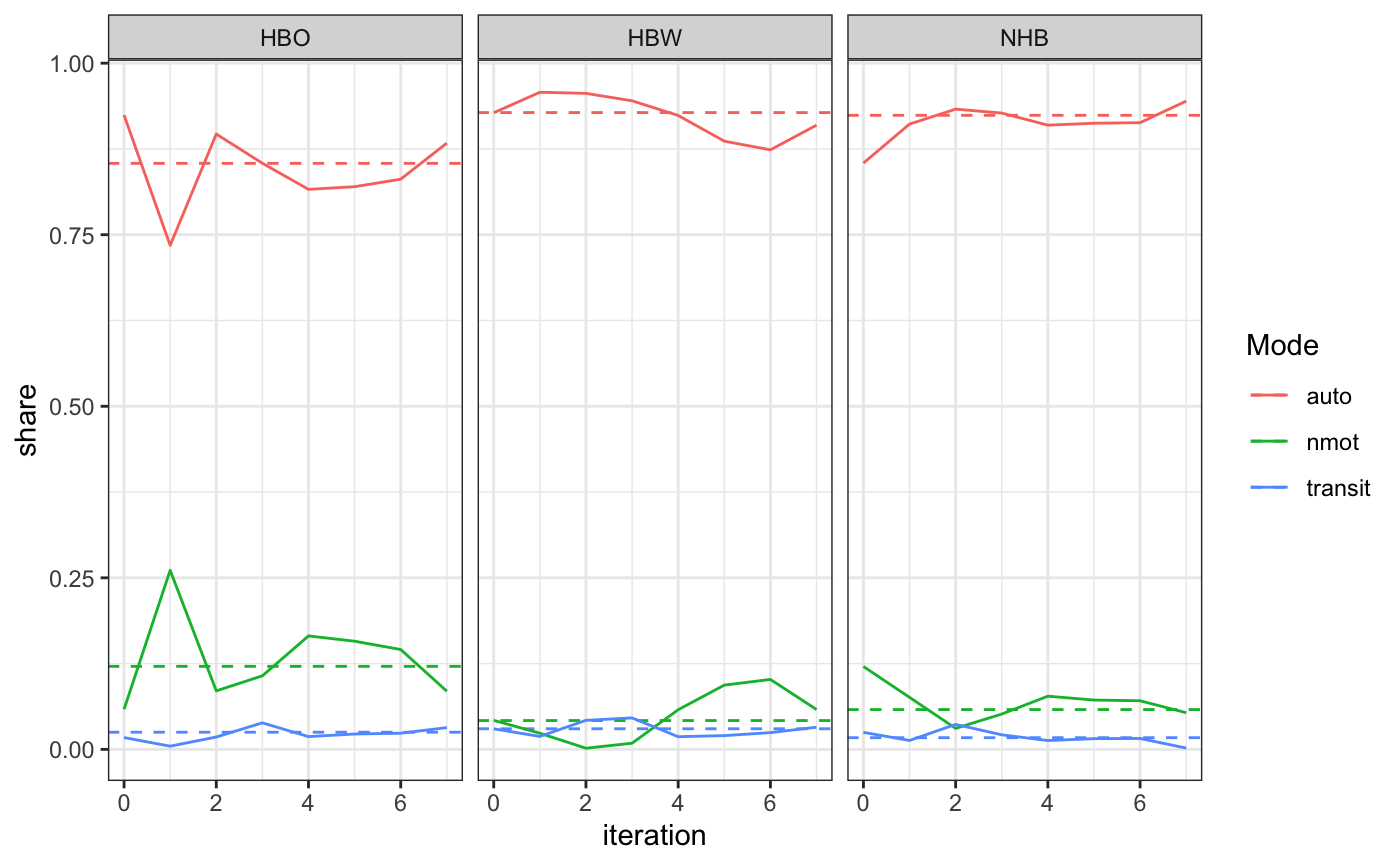
\includegraphics[width=0.75\linewidth]{figures/chapter3/MC_split.png}
  }
  \caption{Mode choice splits by trip purpose; target given by dotten lines.}\label{fig:nhbmc}
  \end{figure}

The DC parameters were also calibrated, however this process differed slightly
from the MC constant calibration process. A destination choice model is also a
multinomial logit model, but this model cannot have alternative-specific
constants because of the high numbers of alternatives (one alternative for
every zone). Instead, the destination choice utility equation can include a
calibration polynomial that adjusts the implied utility to match a trip length
frequency distribution (TLFD) extracted from USTM. In this model, a
cubic polynomial  is included as the destination choice calibration term seen below:
\begin{equation}
  f(d_{ij}) = \kappa_1 d_{ij} + \kappa_2 d_{ij}^2 + \kappa_3 d_{ij}^3
	\label{eqn:poly}
\end{equation}
where $d_{ij}$ represents the distance from $i$ to $j$
and each of the  $\kappa_1,\kappa_2,\kappa_3$, are calibrated to minimize the
difference between the model and target trip length frequency distribution. The target
values for calibration are derived from USTM. The cubic polynomial in
Equation \ref{eqn:poly} --- which is part of the DC utility in
Equation \ref{eqn:dc} --- was applied and calibrated to match the target TLFD
values from USTM. The final calibration values are presented in Table
\ref{tab:coeffs}.

\subsection{Calibration Results}

To ensure that calibration efforts were successful, it was necessary to
compare the TLFD results from USTM and the presented model. A
TLFD script that could divide trips
into distance bins was created. Dividing the trips into distance bins allows for the
breakdown of resiliency trip frequencies by destination, which can then be
compared to the original USTM values. Initial target values for total
trips by purpose were extracted from USTM to ensure that trips in
the presented model were being conserved. Trip totals were compared using
the TLFD outputs to ensure trips of similar lengths were being estimated,
and to the total trips by purpose and mode to ensure trip conservation.

Final trip length distributions for each purpose are similar to the
extracted USTM target values for both the TLFD comparison and the overall
total value comparison. Additionally, Figure \ref{fig:ustm_tlfd} shows the original versus the final
TLFD for the USTM and resilience models. The fit for both is similar, though
there is some variation present between each trip purpose considered.

\begin{figure}

{\centering 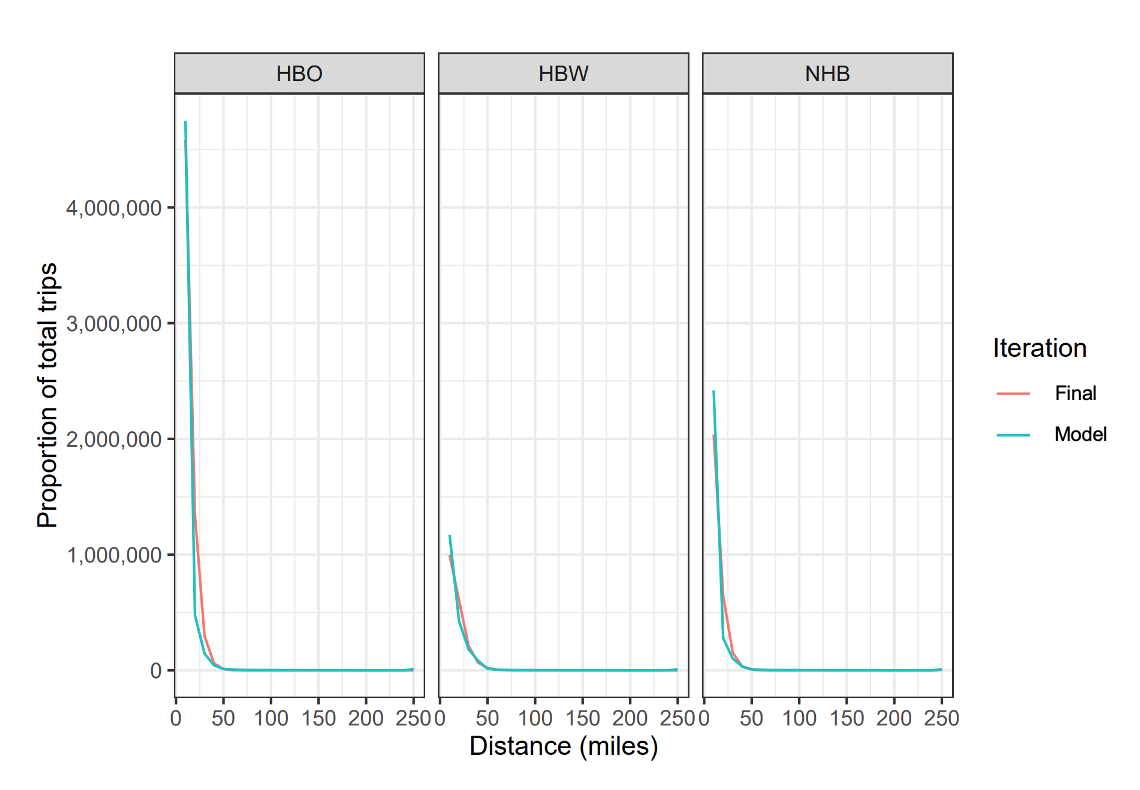
\includegraphics[width=0.75\linewidth]{figures/chapter3/tlfd1.png}

}

\caption{USTM target and final iteration trip length frequency distributions.}\label{fig:ustm_tlfd}
\end{figure}


\section{Method to Calculate Costs for Non-model Purposes}

Some trip purposes contained in USTM did not have enough available data to
include in the logsum portion of the model or did not have
significant impacts and were left out of the logit-based model
calculation. This section will discuss other methods by which costs
associated with each link could be calculated, especially for those
purposes not primarily included in the presented model and for comparison purposes.

Purposes including freight, recreation (REC), and home-based college
(HBC) trips were evaluated using overall travel time change. These
purposes are either rigid in their origins and destinations, as is the
case with most freight trips, or have much smaller frequencies than do the
three main trip purposes HBW, HBO, NHB included in the model. At the same time,
the data needed to create logsum calculations for these
excluded purposes was not readily available. As a result, the costs associated with these trip
purposes was computed based on the increase, or change, in travel time between the base
scenario and an alternative scenario.

The travel time difference is calculated by comparing the change in travel
time between the base scenario and any alternative scenario. The base
scenario highway skim module chooses a route between an OD pair based on
the shortest travel time, not the shortest distance. Thus, the difference
in travel times always remained the same, or increased. The distances, however,
could become shorter, as the shortest distance between an OD pair was not
always the fastest by time. Equation \ref{eqn:time} shows a representation of how
differences in travel time were calculated:
\begin{equation}
	\Delta tt_{ij} = ScenarioTime_{ij} - BaseTime_{ij}
	\label{eqn:time}
\end{equation}
Finding the difference in travel time for each scenario allows for
additional costs to be incorporated that are not included in the logsum
calculation performed on the HBW, HBO, and NHB purposes.

Applying a VOT evaluation, the cost associated with link
closure per day can be measured for each of the purposes not included in
the main logsum analysis. Freight trips and auto trips have different
values of time in USTM, thus the calculated travel time change was
multiplied by different VOTs for each purpose. For passenger vehicle
trips, a VOT of \$17.67 was used, while for freight trips, a VOT of
\$94.04 per hour was used. These values were extracted from USTM and
verified by UDOT's Asset Risk Management Guide \citep{UtahDepartmentofTransportation2020}.
Additionally, the VOT for the logsum method equates to \$16.87 per hour as seen in
Table \ref{tab:VOT}. The method for deriving this value is shown in \ref{eqn:totalcost}.
The auto VOT for the logsum and travel time methods are similar, with a difference
of about \$0.80. The difference in these values would not make an appreciable difference
in the cost estimates between the two methods.

\begin{table}


\caption{\label{tab:VOT}Values of Time for Time Difference Calculations}
\centering
\begin{tabular}[t]{cccl}
\toprule
Freight & Auto & Logsum\\
\midrule
94.04 & 17.67 & 16.87 & Dollars/Hr\\
156.73 & 29.45 & 28.11 & Cents/Min\\
\bottomrule
\end{tabular}
\end{table}

The conversion between the measured DCLS and the actual cost for the logsum method differs from the conversion for the travel time method.
In Table \ref{tab:coeffs}, the coefficient \(\beta_{cost}\) is equal to -0.0016.
To convert between the change in DCLS, or dis-benefit, and the monetary cost to a
single user for each purpose, Equation \ref{eqn:totalcost} must be used.
This gives an estimate of the cost experienced by the whole network as a result
of the closure of a single link.

\section{Summary}

The creation of a logit-based model, which is sensitive to mode and destination
choice, allows for more sensitive and robust estimations of accessibility because
of the ease with which additional data types can be incorporated into the model. The
model also accounts for modes that are not flexible in the case of link
closure. The presented model is capable of analyzing the effects of
road closure on mode and destination choice, and it can estimate overall
dis-benefit (in dollars) experienced by road users per day.

\chapter{Model Application}
\label{chp:chapter4}
\graphicspath{{figures/}{figures/chapter4/}}

\section{Overview}
In this chapter, we apply the Resiliency Model to evaluate the effects of link
loss or degradation on the USTM network. We do this by applying the model to scenarios
where critical highway links have been removed from the USTM network. This
chapter includes first, a detailed analysis of a single scenario, where I-80
between Salt Lake and Tooele Counties is severed. We then compare the model
output to an alternative method that measures only the change in travel
time and does not allow for mode or destination choice. The model was then
applied to 41 individual scenarios, with 40 of those scenarios involving link
closure scenarios throughout the state.

\section{Vulnerable Link Identification}
The methodology developed to identify vulnerable links in Utah uses an online Risk Priority Analysis map created by UDOT to identify points of interest based on existing risk analysis data. Additional
points of interest were identified by the research team or by UDOT officials, who have a familiar working knowledge of the USTM network. Using this
method, links were identified due to their location in relation to
population centers, remote geographic location, proximity to other highway facilities, were known to be at risk due to geologic or geographic features, or
because they were suspected choke points in the network.

After identifying locations of interest, we now apply the model to compare the results of 40 scenarios. In each scenario, an individual highway
facility is removed from the model highway network. Each of these scenario locations is shown in Figure \ref{fig:linksmap}, and is identified in a report by
\cite{aem2017} or the research team using the methodology described. A detailed analysis of the results of a single scenario will be done, followed by a
more general analysis for all 40 scenarios considered in the Resiliency Model.

\section{Localized Scenario Analysis}

This section outlines an in-depth, localized analysis that was conducted to ensure
the Resiliency Model was accurately describing trips likely behavior with OD pairs in the
targeted area around a severed link. This analysis was done on a link between
Tooele and Salt Lake City, Utah. This detailed analysis is useful because it
provides a closer look at the way the Resiliency Model works, capturing trips
between two population centers. Scenario 50, which is located along I-80 between Tooele and Salt Lake Counties
was examined here. The localized analysis shows that the majority of trips
affected by damage to this link either originate or terminate in one of the
two counties, as expected. These results can be seen in Table
\ref{tab:tooeletable}. Another method we used to compare results against is
the travel time method,
which serves to capture trips that have fixed OD pairs such as freight and
recreational trips. This localized analysis also looks at this method.

Table \ref{tab:tooeletable} compares trips and the overall costs between the
logsum and travel time methods, and the specific cost for trips originating in
Tooele County. We can see that the logsum
method captures about
\$123,000 of expenses experienced by road users due to the closure of the
link. Specifically, for trips originating in Tooele County, the logsum based analysis using the Resiliency
Model captures \$1,700 of
expense, which is approximately 1.5\% of the total expense experienced
statewide. A further breakdown of expenses experienced at the local level
for trips originating in Tooele County
can be seen Table \ref{tab:tooeletable}.

The data supports the conclusion that the Resiliency Model is effectively
capturing trips originating in Tooele based on the percent capture
rates in of cost in Table \ref{tab:tooeletable2}. Additionally, when we look at the
travel time method of analysis, we can see that the costs at both the local and
statewide levels are much greater with about \$382,000 and \$437,000
respectively estimated as the costs due to just the increase in travel time, not using
the logit-based model.

\begin{table}
\caption{\label{tab:tooeletable}Localized Analysis Results}

\centering
%\begin{adjustbox}{width=0.9\textwidth}
\begin{tabular}[t]{lrrrr}
\toprule
Trip Purpose & \multicolumn{2}{c}{ \makecell{Whole Network Cost\\ (Dollars per Day)}} & \multicolumn{2}{c}{\makecell{Tooele - SLC Cost \\(Dollars per Day)}}\\
\midrule
 & \makecell{Logsum\\ Method} & \makecell{Travel Time\\ Method} & \makecell{Logsum \\Method} & \makecell{Travel Time\\ Method}\\
\midrule
HBW & \$65,655.13 & \$244,275.72 & \$359.94 & \$12,143.11\\
HBO & \$49,851.54 & \$108,412.94 & \$910.05 & \$3,577.62\\
NHB & \$7,535.78 & \$84,712.36 & \$441.73 & \$5,025.24\\
\midrule
\addlinespace
REC & \$ -  & \$398.72 & \$ -  & \$29.72\\
XXP & \$ -  & \$55,870.17 & \$ - & \$ - \\
Freight & \$ -  & \$10,883,835.01 & \$ -  & \$360,899.92\\
\midrule
HBW, HBO, NHB Total & \$123,042.44 & \$437,401.02 & \$1,711.72 & \$20,745.97\\
Total & \$123,042.44 & \$11,377,504.92 & \$1,711.72 & \$381,675.61\\
\bottomrule
\end{tabular}
%\end{adjustbox}
\end{table}


\begin{table}

\caption{\label{tab:tooeletable2}Localized Analysis Cost Capture Rates}
\centering
\begin{tabular}[t]{ccc}
\toprule
 & Logsum & Travel Time\\
\midrule
HBW & 0.0055 & 0.0497 \\
HBO & 0.0183 & 0.0330 \\
NHB & 0.0586 & 0.0593 \\
\bottomrule
\end{tabular}
\end{table}

The logsum and travel time methods can be broken down into the overall costs and the
comparable costs. The comparable costs are made up of those purposes which are
included in both the Resiliency Model and in the travel time method for determining
cost. HBW, HBO, and NHB trip purposes can be compared because all three trip purposes
are represented by each method of cost estimation.

The travel time method measures the difference in travel time between the base
scenario and any other scenario caused by link closure, and then multiplies that
difference by the VOT for each trip purpose and the number of trips estimated for
each trip purpose. For external trips, freight trips, and REC trips, these were all
extracted directly from USTM. Attempting to include a calculation of the costs
associated with increased travel time for freight trips, external trips, and REC
trips allows a better estimation of the true cost experienced by all road users, not
just those who are included in the Resiliency Model.

The HBW, HBO, and NHB purposes are estimated using the logsum portion of the
Resiliency Model. Calculating the costs associated with the change in logsum
provides estimations of the costs experienced by road users due to link loss
that account for user choice of mode and destination. The logit-based model
employed in the Resiliency Model ultimately provides lower estimates of the
total dis-benefit, and therefore cost, experienced by road users due to link
degradation or loss for the purposes included for analysis. However, the
logsum calculation is only used for three purposes in the USTM model. A way to
account for freight trips, REC trips, and trips that occur between external
nodes must also be found. These trip purposes typically have fixed origins
and destinations. As such, a way to account for all purposes must be developed.
Thus, by combining elements from the travel time method and the Resiliency
Model, an estimate can be made that represents all traffic on the USTM network.

\begin{figure}

{\centering 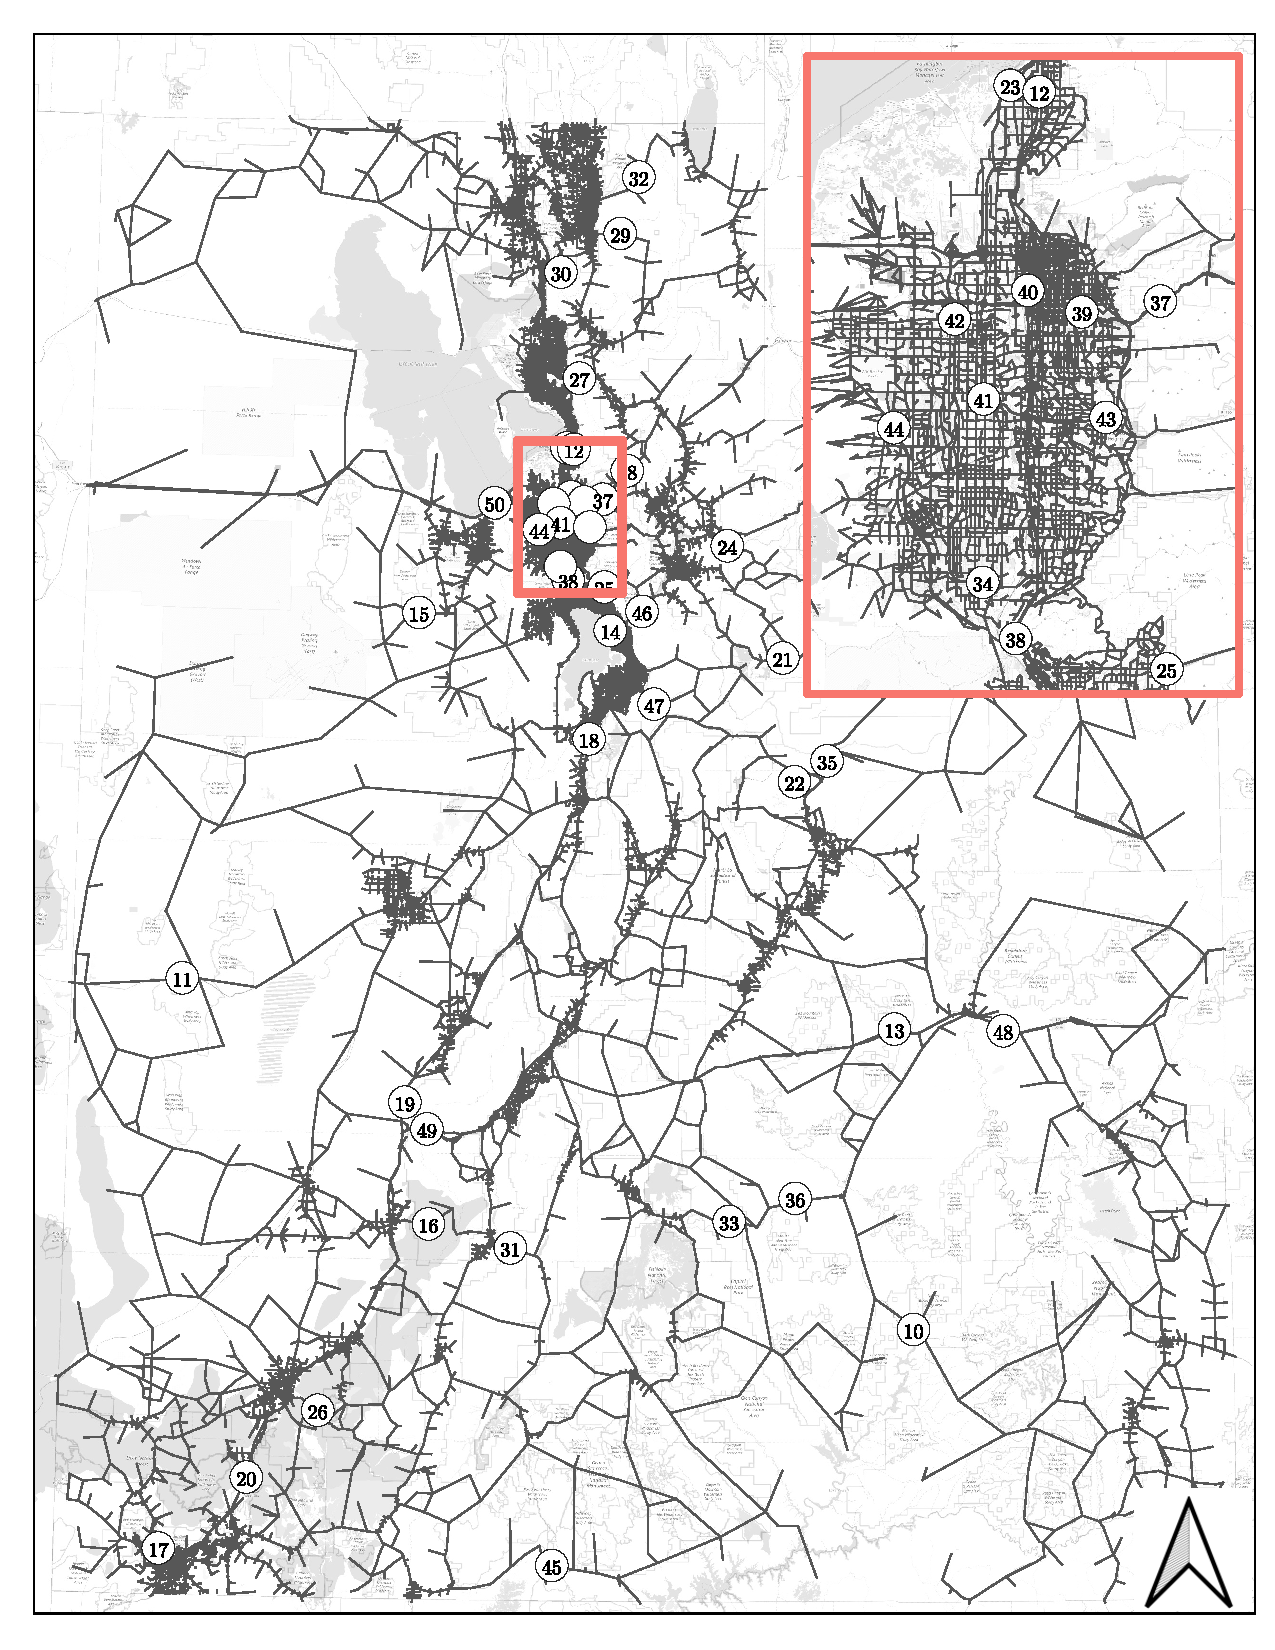
\includegraphics[width=0.95\linewidth]{figures/chapter4/resiliency_links_map.pdf}}

\caption{Links Identified for Analysis.}
\label{fig:linksmap}
\end{figure}

\section{Resiliency Model Results}

The following sections will present the results of the 40 scenarios analyzed.
First, Table \ref{tab:linkresults} shows each of the scenarios we examined,
labeled simply as ``10'' for Scenario 10, and ``11'' for Scenario 11, along with the
change in accessibility, $\Delta$ Logsum, and the Cost Value in dollars per day
associated with link closure. Other identifying information, such as route
numbers or street names and geographic or other identifying descriptions about
the locations where the link was cut, are also provided.

The logsum method results are as follows in Table \ref{tab:linkresults}.
The results are ranked from the road with the largest (most positive
cost) to the road with the smallest cost. We can see that Scenario 27, which
corresponds to I-84 between Ogden and Morgan, experiences the largest cost
per day according to the Resiliency Model. Following Scenario 27, Scenarios 50, 37, 30,
and 17 make up the five most critical roads according to the cost estimation
provided by the Resiliency Model. Each of the roads in these scenarios --- with the exception
of SR-18 in St. George --- is an interstate or state highway facility in
northern Utah, which is heavily populated. Following these five scenarios, are
Scenarios 46, 38, 18, 42, and 41. Each of these facilities are located in northern Utah as well.
Some scenarios, such as Scenario 10,
Scenario 11, or Scenario 33, are roads that are located in remote parts of the state, and
experience no measurable change to HBW, HBO, or NHB traffic. This is
likely due to the remoteness of the geographic location of the highway
link that was cut. A ranking is provided for all of the scenarios examined
using the logsum method in Table \ref{tab:linkresults}.

\begin{table}
\caption{\label{tab:linkresults}Logsum Analysis Results}
\centering
\begin{tabular}[t]{crrll}
\toprule
Scenario & $\Delta$ Logsum & \makecell{Cost \\(per Day)} & Route & Location\\
\midrule
27 & -23830.208 & \$148,938.80 & I-84 & between Ogden and Morgan\\
50 & -19686.788 & \$123,042.42 & I-80 & between SLC and Tooele\\
37 & -8932.691 & \$55,829.31 & I-80 & in Parley's Canyon\\
30 & -7511.948 & \$46,949.67 & US-91 & between Brigham City \& Mantua\\
17 & -5243.828 & \$32,773.92 & SR-18 & just North of St. George\\
46 & -4911.457 & \$30,696.60 & SR-189 & up Provo Canyon near Vivian Park\\
38 & -4422.194 & \$27,638.71 & I-15 & at the Point of the Mount\\
18 & -3186.967 & \$19,918.54 & I-15 & in Rocky Ridge (between Payson \& Nephi)\\
42 & -2657.614 & \$16,610.08 & Bangerter & near West Valley City\\
41 & -1700.167 & \$10,626.04 & I-215 & near Taylorsville\\
25 & -1139.020 & \$7,118.87 & Timp Hwy & at the mouth of AF Canyon\\
24 & -387.467 & \$2,421.66 & UT-35 & outside of Francis\\
23 & -297.882 & \$1,861.76 & Legacy & near West Bountiful\\
20 & -253.712 & \$1,585.70 & I-15 & near New Harmony\\
47 & -142.671 & \$891.69 & US-6 & Spanish Fork Canyon at Diamond Fork Rd\\
26 & -125.740 & \$785.87 & SR-14 & in Cedar Canyon\\
15 & -67.634 & \$422.71 & SR-199 & near Rush Valley\\
32 & -60.883 & \$380.51 & US-89 & between Logan and Bear Lake\\
14 & -45.386 & \$283.66 & I-15 & in Orem between Univ. Ave \& Center St\\
29 & -41.595 & \$259.96 & SR-101 & East of Hyrum\\
31 & -40.108 & \$250.67 & SR-62 & East of Kingston\\
22 & -30.394 & \$189.96 & US-6 & in Carbon County North of Helper\\
49 & -17.768 & \$111.05 & I-70 & near Richfield \& Fillmore\\
45 & -17.029 & \$106.43 & US-89 & near Arizona Border\\
21 & -11.267 & \$70.41 & US-40 & East of Strawberry Reservoir\\
36 & -10.170 & \$63.56 & SR-24 & near Steamboat Point\\
16 & -9.724 & \$60.77 & SR-153 & between Beaver \& Junction\\
48 & -9.717 & \$60.73 & I-70 & near Green River (NW of Moab)\\
19 & -7.623 & \$47.64 & I-15 & near I-70 \& Fillmore\\
35 & -3.762 & \$23.51 & SR-191 & between Helper \& Duchesne\\
13 & -0.135 & \$8.40 & I-70 & at Dragon Point (W of Green River)\\
28 & -0.103 & \$0.64 & SR-65 & border of Salt Lake \& Morgan Counties\\
10 & 0.000 & \$0.00 & SR-95 & near Hite\\
11 & 0.000 & \$0.00 & US-6 & near King Top\\
33 & 0.000 & \$0.00 & SR-24 & in Capitol Reef National Park\\
12 & 894.999 & -\$5,593.74 & I-15 & in Bountiful\\
44 & 2149.291 & -\$13,433.06 & UT-85 & West of West Jordan\\
43 & 4043.132 & -\$25,269.57 & I-215 & near Cottonwood Heights\\
40 & 5576.276 & -\$34,851.72 & I-15 & in SLC between 2100 S \& 1300 S\\
39 & 7434.744 & -\$46,467.15 & I-80 & in SLC near Sugar House and 1300 E\\
34 & 9362.283 & -\$58,514.26 & Bangerter & near Bluffdale\\
\bottomrule
\end{tabular}
\end{table}


\subsection{Scenario Comparison}
Table \ref{tab:comparison} contains a comparison of the results of the logsum
and travel time methods of cost estimation. In the results, we see that the first
a few of the first 10 scenarios differ from the logsum ranking when considering
only HBW, HBO, and NHB as a trip purpose. Scenarios 17, 42, and 46 , which
correspond to SR-18 near St. George, Bangerter Highway near West Valley, and SR-189
near Vivian Park, are among the
most critical facilities in the logsum ranking, but not in the travel time method
for the same trip purposes. The other roads that make up the most critical facilities
for the travel time analysis include Scenarios 18, 27, 30, 37, 38, 41, and 50.
Nearly all of theses scenarios are located in Northern Utah, and are facilities
located on interstate or state highways.

When we consider just those purposes that are a part of the travel time analysis,
but which are not included in the logsum ranking, a few interesting changes occur.
First, Scenario 48 becomes the most critical road due to increased travel time.
Scenario 48 is a facility on I-70 near Green River, Utah.
The other scenarios that comprise the top 10 most critical road segments
in the this analysis are Scenarios 13, 18, 19, 20, 27, 37, 47, 49, and 50. Some
of these scenarios appear in the logsum ranking, and in the travel time method
analysis which only considers HBW, HBO, and NHB trip purposes.

A scenario appearing in more than one result comparison is not unexpected,
because the facilities considered in the Resiliency Model are typically main
arterials in the region where they are located, or are interstate highway
facilities which large amounts of private passenger vehicles and freight.
H ere again, several of the roads that are most critical are located in
Northern Utah. From the travel time method, it is important to note that the main driving factor as to
why a road is important or not closely corresponds closely with
the amount of
freight and external traffic that road experiences along that route. Including freight
trips in the analysis changes the rankings
drastically because of the significantly higher value of time associated
with freight trips.

Some other interesting findings are that in the top 10 most critical scenarios of each analysis
method, three scenarios appear in each of the rankings or comparison rankings. Scenario 18, which is located on
I-15 between Payson and Nephi, Scenario 27 which corresponds to I-
84 in Weber Canyon, and Scenario 37 which corresponds to I-80 in Parley’s Canyon,
are included in the
top 10 scenarios for each of the comparison methods of analysis. This is likely due to the
number of passenger trips along these routes, combined with the number of freight
trips that occur along these routes as well. Interestingly, several of these routes are
the only way through mountain ranges in Utah.

\begin{table}

\caption{\label{tab:comparison} Result Comparison: Logsum vs. Travel Time Method}
\centering
\begin{tabular}[t]{crrrrr}
\toprule
Scenario & \makecell{HBW, HBO, NHB \\ Logsum Method} & \makecell{HBW, HBO, NHB\\ Travel Time Method} & \makecell{Freight, XX Pass, REC\\ Travel Time Method}\\
\midrule
10 & \$0.00 & \$0.00 & \$1,126.41\\
11 & \$0.00 & \$2.83 & \$7,577.46\\
12 & \$(5,593.74) & \$34,668.13 & \$381,210.38\\
13 & \$0.84 & \$3.25 & \$25,310,152.43\\
14 & \$283.66 & \$105,735.73 & \$963,048.78\\
15 & \$422.71 & \$546.85 & \$214.16\\
16 & \$60.77 & \$67.07 & \$30,651.68\\
17 & \$32,773.92 & \$12,151.12 & \$2,086.96\\
18 & \$19,918.54 & \$56,962.31 & \$5,942,067.87\\
19 & \$47.64 & \$150.50 & \$3,478,861.17\\
20 & \$1,585.70 & \$6,722.35 & \$19,531,654.45\\
21 & \$70.41 & \$154.68 & \$541,664.03\\
22 & \$189.96 & \$49.60 & \$688,612.02\\
23 & \$1,861.76 & \$261.55 & \$168.24\\
24 & \$2,421.66 & \$2,952.39 & \$1,885.03\\
25 & \$7,118.87 & \$2,641.43 & \$56.56\\
26 & \$785.87 & \$665.40 & \$751.68\\
27 & \$148,938.80 & \$109,218.22 & \$4,555,377.53\\
28 & \$6.43 & \$0.14 & \$18.65\\
29 & \$259.96 & \$185.03 & \$1.93\\
30 & \$46,949.67 & \$53,897.87 & \$915,569.50\\
31 & \$250.67 & \$965.35 & \$260.08\\
32 & \$380.51 & \$1,457.39 & \$48,530.21\\
33 & \$0.00 & \$7.51 & \$4,113.02\\
34 & \$(58,514.26) & \$34,461.91 & \$19,568.64\\
35 & \$23.51 & \$87.66 & \$184,332.87\\
36 & \$63.56 & \$59.19 & \$1,938.05\\
37 & \$55,829.31 & \$120,030.03 & \$2,066,635.37\\
38 & \$27,638.71 & \$249,676.74 & \$1,752,537.58\\
39 & \$(46,467.15) & \$50,316.65 & \$833,831.51\\
40 & \$(34,851.72) & \$58,824.15 & \$373,714.76\\
41 & \$10,626.04 & \$51,461.48 & \$15,198.52\\
42 & \$16,610.08 & \$15,291.76 & \$4,321.63\\
43 & \$(25,269.57) & \$30,170.94 & \$5,014.80\\
44 & \$(13,433.06) & \$10,701.45 & \$3,498.34\\
45 & \$106.43 & \$495.15 & \$592,294.39\\
46 & \$30,696.60 & \$48,805.90 & \$82,831.00\\
47 & \$891.69 & \$2,473.30 & \$2,044,690.24\\
48 & \$60.73 & \$481.41 & \$85,971,156.40\\
49 & \$111.05 & \$154.96 & \$8,148,497.64\\
50 & \$123,042.42 & \$437,401.02 & \$10,940,103.91\\
\bottomrule
\end{tabular}
\end{table}


\subsection{Positive Benefit Scenarios}

Five of the scenarios indicated a benefit resulting from highway link closure,
which is an unintuitive result. A network should not experience a benefit due
to degradation. As a result, these scenarios were examined more closely to
determine what possible causes could exist behind these atypical and unexpected
results. The affected links are all located in the Salt Lake Valley area at the
following locations: Bangerter Highway near Bluffdale, I-80 near 1300 E, I-15
between 2100 S and 1300 S, I-215 near Cottonwood Heights, Mountain View
Corridor near West Jordan and I-15 near Bountiful.

A discovery made while troubleshooting some calculations is that when a highway link is broken, the new
shortest path by time is longer than in the base scenario with the broken link
available. However, the new path may actually be shorter by distance. This
causes an increase in the utility of accessing destinations by non-
motorized modes, potentially overwhelming the decrease in automobile
utility. It also results in increased auto costs. The automobile accessibility is determined by the AM congested
travel time in the Utah Statewide Travel Model (USTM). The travel distance
– used to determine the accessibility of destinations by driving or
walking – is the distance of that path, and not the actual shortest
distance path. Additionally,
supporting evidence of this theory was found when it was discovered that for
the alternative route between Grouse Creek, Utah, and Salt Lake City,
was nearly twice as long in the case where I-80 was closed between
Tooele and Salt Lake Counties. This discovery led us to understand that not all
route choices become logical when made using only the model data. In
reality, it is possible that a user would find a shorter route
which consists of roads that are not all in the state highway system.

This occurrence is only observed in heavily urbanized regions for two reasons:
\begin{itemize}
	\item The presence of high-speed expressways and parallel local roads
  means that alternate paths with shorter distances but longer vehicle
  times are more likely.
	\item The increased availability of destinations within the non-
  motorized distance threshold (2.5 miles) means that alternative
  destinations exist.

\end{itemize}

Overall, the results of the analysis indicate that the likely cause of a
positive cost being estimated for these five scenarios is that there are
easily
accessible alternate routes in the area, or extremely different alternate
routes along with competing TAZ of similar size in the DC size term
equation.

\section{Summary}

The overall results show that the Resiliency Model is less sensitive to
network changes than the travel time comparison. This is likely because
other behaviors are accounted for in the Resiliency Model. The ability for a user to
choose both a mode and destination (or alternate destination) cause the
logsum results to often estimate a smaller cost than the travel time
results would. However, when the travel time results are factored in, the
overall rankings of the 41 scenarios considered change dramatically. This
is due to the large expenses experienced by freight traffic, which has a
much higher VOT than other passenger trips do. In summary, Table
\ref{tab:linkresults} and Table \ref{tab:timeresults} show the rankings
for both the logsum and travel time analysis methods respectively. The
logsum suggests that I-84 between Ogden and Morgan is the most critical
road, while the travel time method, or total priority, indicates that I-70
near Green River is the most critical road due to cost associated with
closure.

\chapter{Conclusions and Recommendations}
\label{chp:chapter5}
\graphicspath{{figures/}{figures/chapter5/}}

\section{Overview}

This chapter summarizes the recommendations resulting from the resiliency
model application, it also contains information about obtaining the model and
outlines next steps.

\section{Recommendations}

The USTM model is a gravity-based travel demand model, while the Resiliency
Model is logit-based. The logit-based nature of the Resiliency Model allows
for greater sensitivity in user mode and destination choice, which causes
the estimated costs associated with link closure to be lower using the Resiliency Model. The Resiliency
Model's incorporation of both the logsum for HBW, HBO, and NHB purposes, as
well as the travel time calculation for the other purposes included in USTM
provide important functionality towards estimating more realistic, conservative costs
associated with long term highway closure.

Logit-based modeling returns more conservative
estimations of the value of a link in the network. This is a highly
important adaptation to USTM because more accurate and efficient estimation allows
UDOT to better understand the monetary importance of highway links
throughout Utah. Additionally, the model’s design allows for further
analysis of additional link closure, eased identification of critical
points on Utah's highway network, and even multi-link closure in the
future. Thus, it is recommended that USTM include a logit-based mode and destination
choice model in the future.

\section{Limitations and Next Steps}

Implementation of a logit-based travel demand model is highly important for
resource allocation moving into the future. Updating USTM to include a
logit-based trip distribution model instead of a gravity-based model would
improve the flexibility of travel demand estimates moving forward.

The decision to not include a feedback loop, which iteratively runs the model
until a the specifications of a convergence factor are met. Incorporating a
feedback loop would have allowed for more accurate estimation of increased
travel times and more accurate route choices between OD pairs in the final
iteration of the Resiliency model compared with the first iteration.
This decision introduces limitations on the
ability of the model to accurately estimate the effects of link closure on
travel time. This limits the ability of the model to estimate accurate changes in
response to increased travel time due to congestion because cannot be
accurately measured after one iteration.

Adding a congestion feedback loop to the Resiliency Model would allow more
accurate cost estimations to be made. A feedback loop would cause the
travel time and logsum information to be fed back into the beginning of the
model and rerun continuously until the specifications of a convergence
parameter were met. The loop would allow for better estimates of the change
in travel time due to both route change and resulting congestion. The loop
also allows for more accurate route choice, mode choice, and destination
choice to be made when the true effects of congestions are accounted for.
In June 2020, the UDOT Technical Advisory Committee decided to not include a
feedback loop to save time
on model development for this study. A feedback loop and sensitivity analysis
should be included as part of future work.

It is not unreasonable to assume that in the event of an earthquake or
similar widespread disaster event, that multiple links could become
damaged. An important use of the Resiliency Model in future research would be
to analyze the results of simultaneous multiple link
loss. This will allow for
greater understanding of the effects that adverse events can have on Utah’s
highway network, and help UDOT to better prepare for the development and
maintenance needs of the future. Developing a fully functioning transit oriented logit model
would be highly advantageous to the Utah Transit Authority as well. The capability
is already incorporated into the structure of the resiliency model, however, a few modifications
need to be made in order for it to become fully functioning.
Additionally, the development of logsum calculations for trips with fixed
origins and destinations should also be considered. This model, however,
would be very different than the Resiliency Model because freight trips
do not typically have a mode or destination choice option, so it would be
more prudent to be able to account for other choices such as travel time,
distance or even elevation change on a given route. One option is to use the national
freight network, which would allow freight trips to divert through other Interstate
facilites.

\section{Summary}

The development of a logit-based travel demand model can improve the
ability of UDOT to accurately estimate the costs per day of link loss that
Utahns would experience. The Resiliency Model provides sensitive
estimates that more accurately represent the costs associated with link
closure than a travel time increase methodology by itself would be able to
capture. Using the logsum, estimations sensitive to user choice were
found, which can help professionals to better evaluate risk to Utah’s
infrastructure. User choice is highly important in modern modeling
practices because user choice allows a model to estimate information more
precisely while accounting for the ability of a user to choose. The information
provided by the Resiliency Model
should be used to prioritize link importance to the functionality of
Utah’s highway network. The Resiliency Model provides different estimates of
costs experienced by Utahns due to link loss than traditional methods for
determining costs do. There are several implications of this. First, purely
using change in travel time or travel time delay as the main dis-benefit may not
be entirely accurate in most situations. Second, allowing users in the model
to choose both a mode and destination, increases the resemblance of a real life
decision making process, especially given adverse circumstance on Utah's
highway network. It is evident that the Resiliency Model provides several
modeling estimation advantages to the forefront, something which must be
explored further in future research.


%%%%%%%%%%%%% begin Bibliography %%%%%%%%%%%%%%%%%
\cleardoublepage
\bibliographystyle{apalike}%Change this to use a different bibliography
%style, such as ieeetran.
\bibliography{refs}% Change this to use a different bibliography database
%file.

% Include appendix sections here: (or comment these lines out to have no
%appendices)
%\appendix
%\chapter{Making a Figure with Width Based on Page Size}
\label{apdx:appendixa}
\graphicspath{{figures/}{figures/appendixa/}}

\section{Width Based on Page Size Figure Example} \label{sec:appendixa_figure_example}
Here's an example of a figure whose width depends on the width
of the page. You can see it as Figure~\ref{fig:appendix_some_pic}. This also shows another citation \cite{aeyels86local}.

\begin{figure}[htbp]
  \centering
  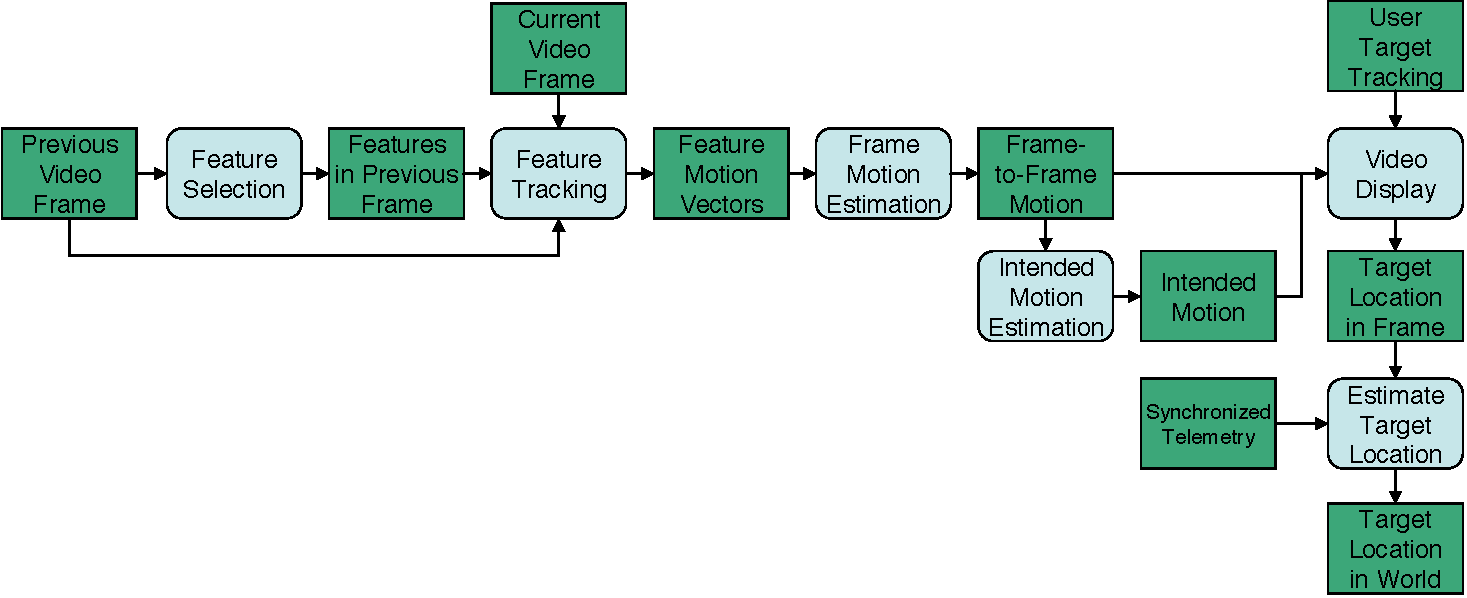
\includegraphics[width=0.45\textwidth]{some_pic}
  \caption[Example figure whose width depends on page size]{
    This is an example of a figure whose width will be 45\% of the
    width of the page. If you'd like to see a figure with a fixed
    width then you can see it as Figure~\ref{fig:intro_stuff} in
    Section~\ref{sec:intro_figure_example} of Chapter~\ref{chp:chapter1}.}
  \label{fig:appendix_some_pic}
\end{figure}
%\chapter{Formatting Guidelines for Thesis}
\label{apdx:appendixb}

This appendix outlines the required formatting for theses and dissertations. While the \LaTeX\ template takes care of most of these automatically, it is the student's responsibility to ensure that all formatting requirements are incorporated in the document.

\section{Font} Times New Roman 12 pt. throughout text and 10 or 11 point for tables and figures.

\section{Margins}
\begin{itemize}
\item Preliminary Pages (Title page, Abstract page(s), Acknowledgment page, Table of Contents, List of Figures, List of Tables):
1 inch on all sides
\item Body Pages, beginning with Introduction:
1 inch on all sides
\item Chapter title pages, Appendix title page, Reference title page:
2 inches at top,
1 inch at bottom and sides
\end{itemize}

\section{Printing}
\begin{itemize}
\item Single-sided: Title page, Abstract page(s), Acknowledgment page
\item Two-sided:  Table of Contents, List of Figures, List of Tables, Body, Appendix, References
\end{itemize}
Note:  Table of Contents, List of Figures, List of Tables, Chapter title pages, References and Appendix pages must begin on the front side of a page.

\section{Page Numbering}
\begin{itemize}
\item	Page numbers are centered at the bottom of the page.
\item	Counting begins with the Title page; however, back pages are not counted until the Table of Contents.
\item	Page numbers do not appear on the page until the Table of Contents (v).
\item	Use Roman Numerals (v, vi, vii, ...) for the Table of Contents page and the pages thereafter until Chapter 1.  
\item	Use Arabic numbers (1, 2, 3 ...) beginning with Chapter 1. 
\item	Be sure numbers appear on all blank back pages once numbering begins.
\end{itemize}

\section{Spacing}
\begin{itemize}
\item	Double-space text of body.
\item	Single-space abstract, captions, quotes, long chapter titles, headings, and subheadings.
\item	Table of Contents, List of Figures, List of Tables, and References can be single-spaced or double spaced.
\item	Double-space three times after chapter titles (48 pts).
\item	Double-space twice before subheadings (24 pts). 
\item	Double-space once after subheadings (0 pts). 
\item	Double-space once between two subheadings (0 pts). 
\item	Double-space twice before and after figures (24 pts).
\item	Double-space twice before and after tables (24 pts).
\item	Double-space once before and after equations (0 pts).
\item	Do not leave a single line of text, a single-line equation, or a subheading alone on the top (widow) or bottom (orphan) of a page.
\item	Do not leave more than about 5 lines of white space remaining on a page unless it�s the end of a chapter.
\end{itemize}

\section{Figures}
\begin{itemize}
\item	Figures are normally diagrams, graphs, maps, or charts.
\item	Center figures on the page.
\item	Center captions below the figure. If two lines are needed, the caption should be left justified at margin.
\item	A figure should be placed after the paragraph of reference.  If it will not fit on the same page, continue the text and place the figure on the next page.
\end{itemize}

\section{Tables}
\begin{itemize}
\item	Tables contain numerical or statistical information.
\item	Center tables on the page.
\item	Center captions above the table.  If more than one line is needed, center the lines in an inverted pyramid:                                                          
\begin{singlespace}
\begin{center}Table 6.3 Comparison of roll rotation plots when node was displaced,\\
 and an X-direction off-axis force was applied.\end{center}
\end{singlespace}
\item	If placed in the landscape position, the top of the table should be on the left side of the page, with the caption above the table.  The page number is placed in the standard location.
\end{itemize}

\end{document}
